\documentclass[a4paper,10pt,openany,oneside]{report}

\usepackage{amsfonts}
\usepackage{pstricks}
\usepackage{amsmath}
\usepackage{amssymb}
\usepackage[french]{babel}
\usepackage{changepage}
\usepackage{color}
\usepackage{enumitem}
\usepackage{fancyhdr}
\usepackage[T1]{fontenc}
\usepackage[left=2cm,right=2cm,top=1.5cm,bottom=1.5cm,headsep=1cm,includefoot]{geometry}
\usepackage{graphicx}
\usepackage[hidelinks]{hyperref}
\newcommand{\link}[1]{{\color{blue}\href{#1}{#1}}}
\usepackage[utf8]{inputenc}
\usepackage{listings} %Pour le code
\usepackage{titlepic}
\usepackage{wrapfig}
\usepackage{longtable}
\usepackage[]{algorithm2e}
\usepackage{makecell}
\renewcommand\theadfont{\bfseries}
\usepackage{float}
\usepackage{parskip}
\usepackage{pdfpages}
\usepackage{caption}

\newcommand{\source}[1]{\caption*{Source: {#1}} }


\setitemize{topsep=5pt}
\setlength{\parindent}{1em}
\setlength{\parskip}{1em}

\definecolor{dkgreen}{rgb}{0,0.6,0}
\definecolor{gray}{rgb}{0.5,0.5,0.5}
\definecolor{mauve}{rgb}{0.58,0,0.82}
\definecolor{myblue}{rgb}{0,0,1}
\definecolor{bonus}{rgb}{1,0.7,0}

\newcommand\blfootnote[1]{%
  \begingroup
  \renewcommand\thefootnote{}\footnote{#1}%
  \addtocounter{footnote}{-1}%
  \endgroup
}
\makeatletter
\renewcommand{\@makeschapterhead}[1]{%
%  \vspace*{50\p@}%
  \vspace*{35\p@}%
  {\parindent \z@ \raggedright
    \normalfont
    \interlinepenalty\@M
    \Huge \bfseries  #1\par\nobreak
%    \vskip 40\p@
    \vskip 20\p@
  }} 
  
\lstset{frame=tb,
  language=python,
  aboveskip=3mm,
  belowskip=3mm,
  showstringspaces=false,
  columns=flexible,
  basicstyle={\small\ttfamily},
  numbers=left,
  numberstyle=\normalsize,
  numbersep=7pt,
  numberstyle=\tiny\color{gray},
  keywordstyle=\color{blue},
  commentstyle=\color{dkgreen},
  stringstyle=\color{mauve},
  breaklines=true,
  breakatwhitespace=true,
  tabsize=4,
}

\lstset{frame=tb,
  language=python,
  aboveskip=3mm,
  belowskip=3mm,
  showstringspaces=false,
  columns=flexible,
  basicstyle={\small\ttfamily},
  numbers=none,
  numberstyle=\normalsize,
  numbersep=7pt,
  numberstyle=\tiny\color{black},
  keywordstyle=\color{black},
  commentstyle=\color{black},
  stringstyle=\color{black},
  breaklines=true,
  breakatwhitespace=true,
  tabsize=4,
}

\begin{document}
\pagenumbering{gobble}
\vspace*{1cm}
\begin{figure}
	\centering
	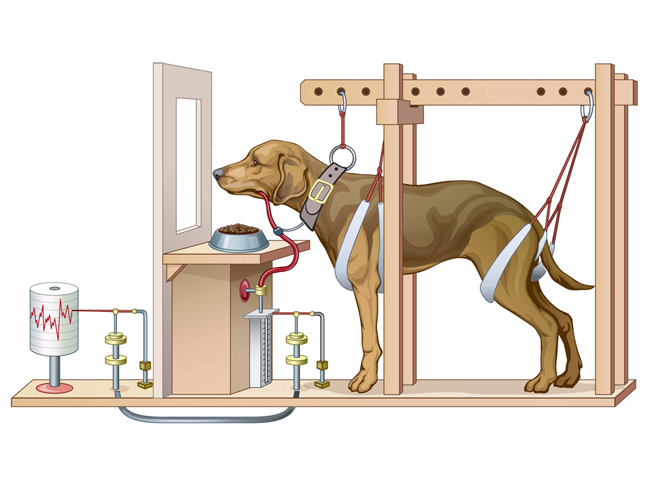
\includegraphics[scale=0.5]{img/pavlovs_dog.jpg}
\end{figure}
\vspace*{2cm}
\begin{center}
	\textbf{\Huge Reinforcement Learning} \\[1cm]
	\textbf{\Huge Travail d'automne} \\[0.5cm]
	{\Large Sergiy Goloviatinski, inf3dlm-b\\2018-2019, HE-Arc\\Numéro de projet 212}
	\\[4cm]
	25 janvier 2019
\end{center}

\setcounter{tocdepth}{3}
\setcounter{secnumdepth}{3}

\chapter*{Abstract}
\thispagestyle{empty}
\subsubsection*{Français}
Ce rapport présente le déroulement d'un projet de semestre effectué à la HE-Arc qui consistait à développer un module python permettant de faire du Reinforcement Learning avec des approches de deep Q-Learning.

Une grande partie de ce projet était l'apprentissage des techniques de Reinforcement Learning et ensuite de l'exploration afin d'améliorer les résultats dans un scénario donné.

Deux scénarios ont été utilisés pour tester l'efficacité de l'IA ainsi développée:
\begin{itemize}
\item Le jeu vidéo Doom, où le but était de survivre le plus longtemps possible face à des vagues d'ennemis sur lesquels l'IA devait tirer.
\item Le jeu vidéo Flappy Bird où le but pour l'IA était d'arriver le plus loin possible dans le jeu en sautant pour évoluer dans le niveau en évitant de s'écraser contre les tuyaux.
\end{itemize}


Les résultats obtenus ont été convaincants: dans Doom, l'IA a développé un comportement où elle visait les ennemis apparaissant et leur tirait dessus, et dans Flappy Bird l'IA a réussi à trouver comment doser les sauts pour passer au mieux entre les tuyaux.


Mots-clés: intelligence artificielle, IA, Reinforcement Learning, RL, Doom, Flappy bird, Q-Learning, python, tensorflow, keras-rl, VizDoom, PLE, Py Learning Environment
\subsubsection*{English}
This report presents the progress of a semester project carried out at HE-Arc, which consisted in developing a python module to make Reinforcement Learning with deep Q-Learning approaches.

The bulk of this project consisted in learning Reinforcement Learning techniques and then exploring to improve results in a given scenario.

Two scenarios were used to test the effectiveness of the developed AI:
\begin{itemize}
	\item The video game Doom, where the goal was to survive as long as possible against waves of enemies on which the AI had to shoot.
	\item The video game Flappy Bird where the goal for the AI was to get as far as possible in the game by jumping to evolve in the level and avoiding crashing against the pipes.
\end{itemize}

The results were convincing: in Doom, the AI developed a behavior where it targeted the enemies appearing and shot at them, and in Flappy Bird the AI managed to find out how to gauge the jumps to pass between the pipes in the best way possible.

Keywords: artificial intelligence, AI, Reinforcement Learning, RL, Doom, Flappy bird, Q-Learning, python, tensorflow, keras-rl, VizDoom, PLE, Py Learning Environment
\pagebreak

\tableofcontents

\setcounter{page}{0}
\pagestyle{headings}
\renewcommand{\@makeschapterhead}[1]{%
%  \vspace*{50\p@}%
  \vspace*{50\p@}%
  {\parindent \z@ \raggedright
    \normalfont
    \interlinepenalty\@M
    \Huge \bfseries  #1\par\nobreak
%    \vskip 40\p@
    \vskip 40\p@
  }} 
\chapter{Introduction}
\pagenumbering{arabic}
\thispagestyle{headings}
\begin{figure}[H]
	\centering
	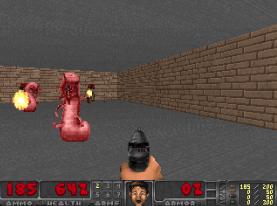
\includegraphics[width=0.4\textwidth]{img/doom.png}
	
\includegraphics[width=0.3\textwidth]{img/flappybird.png}
	\caption{A gauche: le jeu vidéo Doom, à droite: le jeu vidéo FlappyBird, tous les deux ont pu être jouables par une IA grâce aux techniques de Reinforcement Learning}
\end{figure}
\section{Qu'est-ce que le Reinforcement Learning ?}
Le Reinforcement learning (apprentissage par renforcement en français), est une technique utilisée en intelligence artificielle consistant à faire apprendre à une IA  quelles actions  entreprendre selon l'état de l'environnement au moment d'entreprendre cette action, afin de maximiser un score.\cite[]{wikipediaRL}

Pour que cette technique fonctionne, il faut un environnement capable de recevoir des actions à entreprendre et retournant un état et une récompense issue de l'action entreprise précédemment au sein de cet environnement.

Le but de l'agent est de maximiser la somme des récompenses ainsi obtenues, pour ce faire il y a plusieurs algorithmes et façons de prédire la récompense que donnera une action en se basant sur des expériences passées.
\begin{figure}[H]
	\centering
	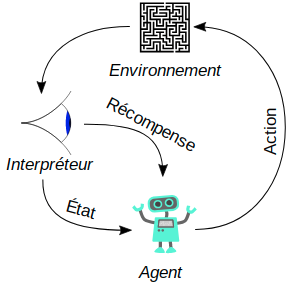
\includegraphics[width=0.4\textwidth]{img/rl_schema.png}
	\caption{Illustration du principe de base du reinforcement learning \cite[]{wikipediaRL}}
	\source{rwikipedia}
\end{figure}
\subsubsection*{Quelques précisions relatives aux termes utilisés}
\begin{description}
	\item[Agent:] Un acteur qui entreprends des actions en agissant, une IA dans le cas du Reinforcement Learning
	\item[Action:] Action possible à entreprendre dans un contexte donné, par exemple sauter, avancer, tirer dans un jeu-vidéo
	\item[Récompense/score:] Comme un score qu'un joueur gagnerait dans un jeu-vidéo ou comme une récompense comme de la dopamine dans le cerveau
	\item[Environnement:] Entité avec laquelle l'agent interagit en y effectuant des actions (p. ex un jeu-vidéo, une simulation, le monde réel) 
	\item[Etat:] Interprétation de l'environnement en tant que vecteur caractéristique ou les pixels affichés à l'écran 
	\item[Politique:] Règles guidant des décisions afin d'atteindre un résultat voulu 
	\item[Interpréteur:] Entité qui permet d'interpréter l'environnement afin de le représenter avec un état sous la forme qu'attends l'algorithme de Reinforcement Learning, de plus l'interpréteur décide si le changement de l'environnement a provoqué une récompense (positive ou négative) ou non (il est à noter que dans certains frameworks de Reinforcement Learning, l'interpréteur est intégré à l'environnement)
\end{description}

Beaucoup de ces termes viennent de ce qu'on appelle "processus de décision markovien" ou "modèle de Markov", qui est un modèle développé dans les années 1950 dans le cadre d'une discipline appelé "théorie de décision" permettant de modéliser des systèmes qui changent aléatoirement. Dans le cadre de ce modèle, un agent prends des décisions et les résultats de ses actions sont aléatoires. A chaque étape, le processus est dans un certain état, et l'agent choisit une certaine action qui rapportera une certaine récompense à l'agent.

\section{Utilisations et prouesses du Reinforcement Learning}
\begin{figure}[H]
	\centering
	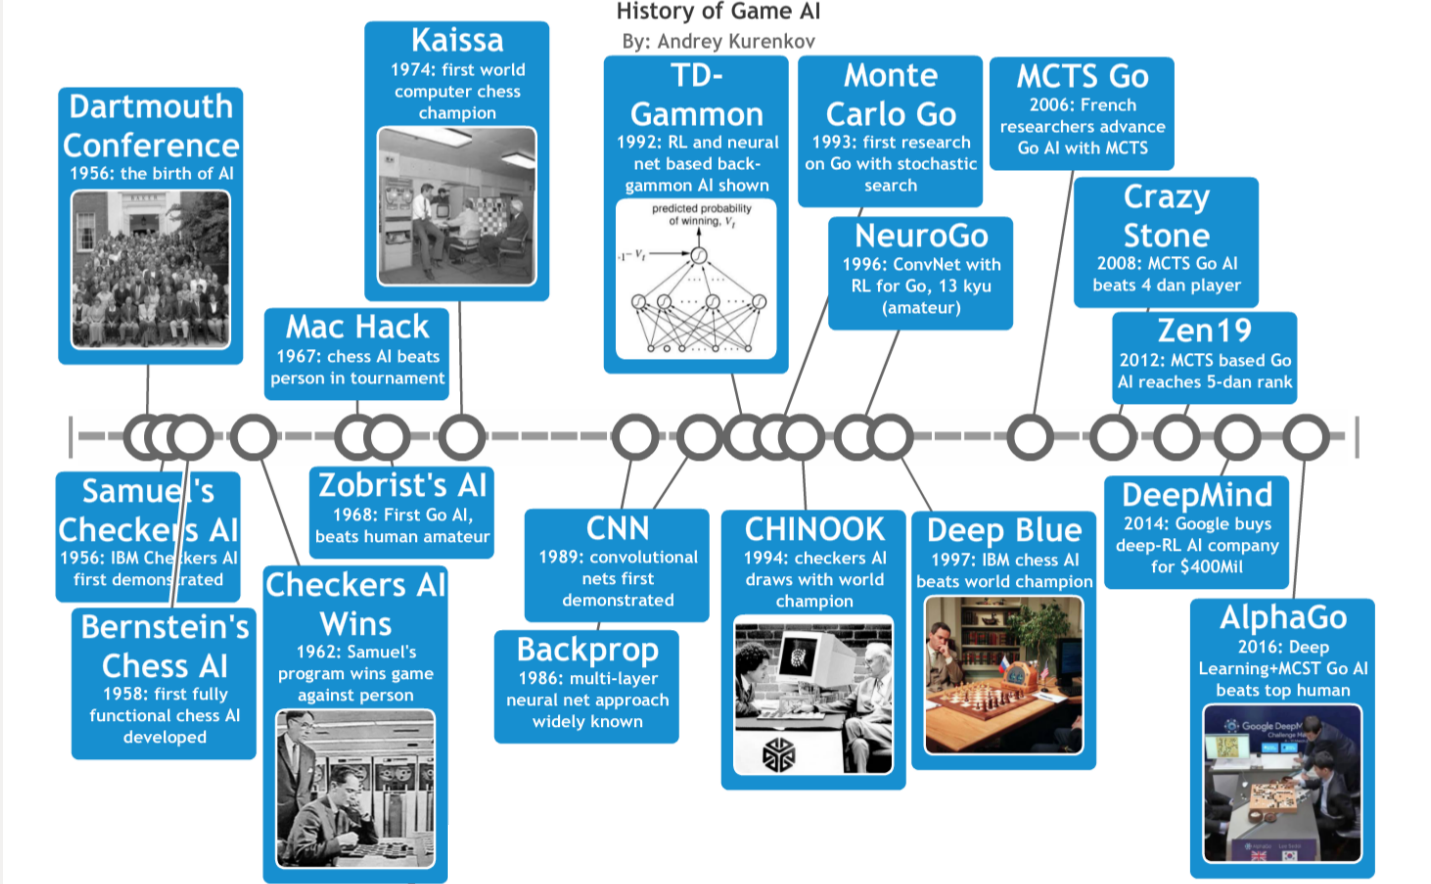
\includegraphics[width=0.8\textwidth]{img/histoire.png}
	\caption{Différentes étapes dans l'histoire des IA de jeux jusqu'en 2016, à noter AlphaGo qui se situe tout à droite et que depuis il y a encore eu du progrès \cite[]{andreykurenkov}}
\end{figure}
Le Reinforcement Learning avait beaucoup fait parler de soi quand l'IA mis au point par DeepMind (l'IA s'appelait AlphaGo) a battu le champion du monde dans le jeu de Go en 2016.

Récemment, un projet nommé "OpenAI Five" a mis au point une équipe de 5 bots collaborant entre eux pour jouer au jeu vidéo "Dota 2", pour l'instant ils ont réussi à battre des équipes de joueurs amateurs mais cela est considéré comme une grande prouesse car ce jeu est considéré comme étant complexe pour une IA à cause de la collaboration requise entre joueurs pour gagner une partie.

Le reinforcement learning est aussi utilisé dans le cadre des voitures autonomes, pour cela il est possible d'utiliser un jeu-vidéo comme "GTA V" en tant que simulation avant d'appliquer un modèle ainsi entraîné dans la vraie vie.
\section{Différents algorithmes de Reinforcement Learning utilisés dans ce projet}
\subsection{Q-Learning}
Le Q-Learning est une méthode d'apprentissage utilisé dans le Reinforcement learning. La lettre "Q" (comme "Qualité") désigne la fonction qui prédit la qualité d'une action exécutée dans un état donnée du système en se basant sur des expériences passées. La valeur de sortie de cette fonction est désignée "Q-value" \cite[]{wikipediaRL}

Le but du Q-Learning est d'apprendre une politique qui dit à l'agent quelle action entreprendre selon quelle circonstance. Pour cela on n'a pas besoin d'un modèle de l'environnement établi préalablement.

Le Q-Learning trouve une politique qui est optimale dans le sens où elle maximise la valeur attendue de la somme de récompense sur toutes les étapes successives.
\newpage
Voici la définition formelle de cette fonction:
$Q[s, a] := (1-\alpha)Q[s, a] + \alpha(r+\gamma max_{a'}Q[s', a'])$

\begin{itemize}
	\item s est un état (state)
	\item a est une action
	\item r est la récompense liée à ce couple état-action
	\item $\alpha$ est le facteur d'apprentissage (learning rate), il détermine à quel point la nouvelle information calculée surpassera l'ancienne. Un facteur de 0 ne ferait rien apprendre à l'agent, alors qu'un facteur de 1 ne ferait considérer à l'agent que la dernière information. Une valeur proche de 1 est optimale dans un environnement déterministe
	\item $\gamma$ est le facteur d'actualisation (discount rate), il détermine l'importance des récompenses futures. Un facteur 0 ferait considérer que les récompenses courantes à l'agent, et un facteur proche de 1 ferait intervenir les récompenses lointaines.
\end{itemize}
\begin{figure}[H]
	\centering
	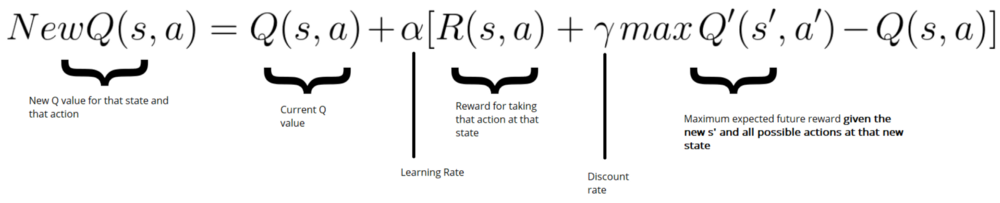
\includegraphics[width=1\textwidth]{img/qfunction.png}
	\caption{Explication visuelle de la fonction Q \cite[]{freecodecamp}}
\end{figure}

En pratique, pour implémenter cette méthode on utilise un tableau à 2 dimensions (appelée "Q-Table"), où un indice représente un état et l'autre indice représente une action et la case de la matrice liée à une action combinée avec un état contiendra le résultat de la fonction "Q".

\begin{figure}[H]
	\centering
	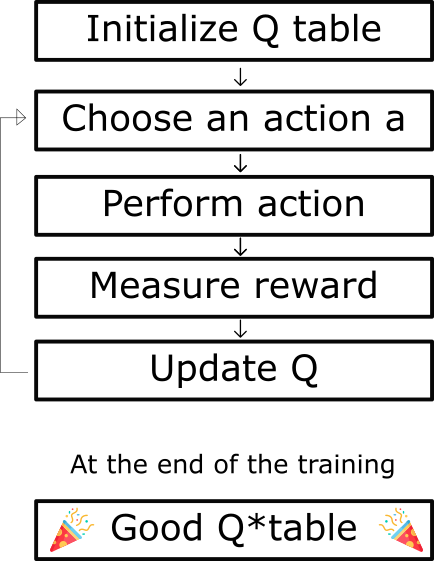
\includegraphics[width=0.3\textwidth]{img/qtable.png}
	\caption{Schéma expliquant les actions à entreprendre lors d'un remplissage d'une Q-Table en pratique \cite[]{freecodecamp}}
\end{figure}

Cette technique est viable dans un cas où l'espace d'actions et d'états possible n'est pas "trop" grand (car le tableau bidimensionnel aura une taille de $A*S$ avec $A$ le nombre d'actions possibles et $S$ le nombre d'états possibles), dans un cas où l'état serait représenté par des pixels, cette solution n'est plus valable car il y aurait beaucoup trop d'états possibles et le tableau bidimensionnel contenant les Q-Values serait trop grand pour être stocké dans la mémoire d'un ordinateur.
\subsection{Deep Q-Learning (DQN)}
Afin de pouvoir appliquer le Q-Learning à des scénarios ayant un vaste espace d'états, une solution est d'utiliser un réseau de neurones qui va approximer pour un état donné, les différentes Q-values pour chaque action possible.\cite[]{freecodecamp}

Grâce à l'utilisation des réseaux de neurones, on n'est plus obligé de stocker tous les tuples état-action dans un tableau bidimensionnel, mais on peut utiliser le réseau de neurones pour approximer une fonction qui donnerait une Q-Value pour un état donné, et le résultat de cette approximation sera stocké dans une mémoire avec les poids des neurones correspondant à chaque état.

\begin{figure}[H]
	\centering
	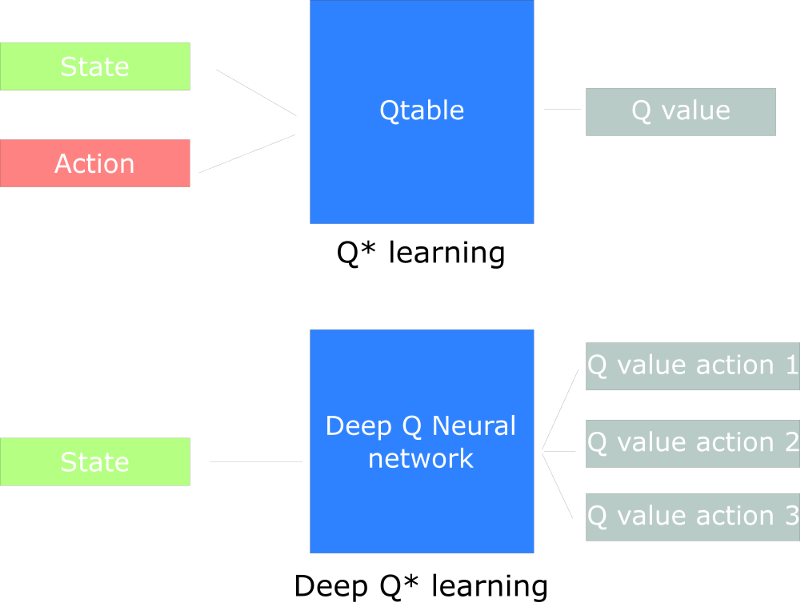
\includegraphics[width=0.5\textwidth]{img/qtable-dqn.png}
	\caption{Schéma illustrant le changement entre le Q-Learning et le Deep Q-Learning \cite[]{freecodecamp}}
\end{figure}

Qu'est-ce qu'un réseau de neurones? Dans le cadre de l'IA, un réseau de neurones est composé de neurones disposés en couches, et les neurones d'une couche sont reliés aux neurones de la couche suivante. Chaque couche traite les informations de la couche précédente et les transmets aux couches suivantes.
\begin{figure}[H]
	\centering
	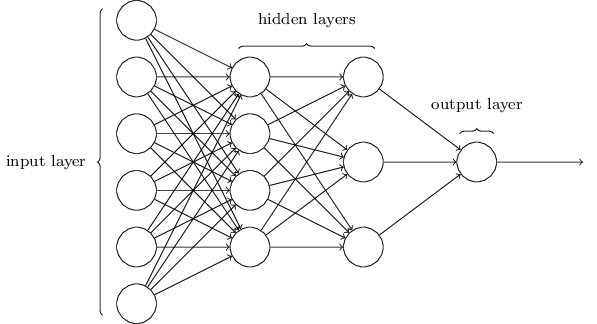
\includegraphics[width=0.6\textwidth]{img/neuralNetwork.png}
	\caption{Schéma illustrant l'architecture et la propagation d'informations dans un réseau de neurones \cite[]{neuralnetworksanddeeplearning}}
\end{figure}
Dans le cas du deep Q-learning, le réseau aura en entrée un état, et en sortie une Q-value associé par état possible.

A force de faire des expériences, l'agent nourri le réseau de neurones et l'approximation de la Q-value devient de mieux en mieux en réduisant l'erreur entre la valeur prédite et la valeur maximale possible du prochain état ("Q-Target").

Cette approche permet d'intégrer des couches de neurones convolutifs à l'entrée du réseau, permettant de traiter des états issus de pixels, comme dans le cas d'un jeu-vidéo comme doom. Sans l'utilisation de réseaux de neurones ceci ne serait pas possible.

Un soucis de cette technique est que les poids reliant les neurones entre eux ne sont que valables pour un état donné, donc quand on change d'état, les poids doivent s'adapter et le réseau "oublie" les poids des états précédents.

Pour corriger ce soucis, nous avons besoin d'une mémoire qui stocke les expériences précédentes, et on utilisera des échantillons pris de façon aléatoire parmi les expériences passées pour nourrir notre réseau de neurones. Ceci permettra au réseau de neurones d'apprendre sur le long terme en se basant sur une large gamme d'expériences effectués par l'agent et ne pas apprendre seulement en se basant sur les expériences les plus récentes. Cette mémoire s'appelle "replay buffer".
\subsection{Améliorations du deep Q-Learning}
Depuis l'introduction du deep Q-Learning en 2014, plusieurs améliorations ont été mises au point pour pallier à certains points faibles que contenait cette technique, les sections suivantes présentent quelques unes qui ont été utilisés dans le cadre de ce projet.
\subsubsection{Fixed Q-targets}
Afin de réduire la marge d'erreur entre la prédiction de la Q-value et la Q-target (valeur maximale possible pour le prochain état), on calcule la différence entre la prédiction et la vraie valeur. Sauf que, la prédiction n'est qu'une estimation de la Q-value. Mais la valeur estimée et la vraie valeur sont issus du même réseau de neurones, donc il y a une forte corrélation entre les deux. Ce qui veut dire qu'à chaque nouvelle étape de l'entraînement, un décalage de la vraie valeur entraîne un décalage de l'estimation ce qui entraîne une oscillation de la marge d'erreur pendant l'entraînement.

Une solution à ce problème à été proposée par DeepMind: utiliser un réseau de neurones séparé avec un paramètre fixe pendant une certaine période pour estimer la Q-value. Grâce à ça, la phase d'apprentissage sera plus stable car la Q-value estimée reste la même pendant un moment.
\subsubsection{Double DQN}
Un autre problème du DQN est la possibilité de surestimer la Q-value, et on n'est plus sûr que la meilleure action à entreprendre dans un état donné est forcément celle qui a la plus haute Q-value.

Ce problème survient surtout au début de l'entraînement, lorsque on ne dispose pas d'assez expériences pour pouvoir choisir la meilleure action à entreprendre.

La solution à ce problème est d'utiliser le 2ème réseau de neurones introduit par la solution des fixed Q-targets afin de découpler le choix de l'action de la génération de l'estimation de la Q-value. Pour cela nous utiliseront le réseau principal pour sélectionner la meilleure action à entreprendre pour un état donné basé sur la plus haute Q-value, et le second réseau pour estimer la Q-Value au prochain état si cette action sera prise. Ceci permet de réduire sur surestimation de la Q-Value et donc permet d'avoir un entraînement plus stable et rapide.
\subsubsection{Dueling DQN}
Une Q-value représente à quel point entreprendre une action dans un état donnée nous sera favorable, donc on peut décomposer $Q(s,a)$ en: $Q(s,a) = A(s,a) + V(s)$ , avec $V(s)$ la Q-valeur en étant à cet état et $A(s,a)$ le gain (advantage) qu'on aura en prenant cette action dans cet état, ou à quel point cette action nous rapportera plus que les autres actions possibles à cet état.

Le principe du dueling DQN est de séparer l'estimation de ces deux éléments avec deux flux: un qui estime la valeur lié à un état $V(s)$ et un autre qui estime le gain de chaque action $A(s,a)$

Ensuite, ces deux flux seront combinés pour finalement donner une estimation de $Q(s,a)$.
\begin{figure}[H]
	\centering
	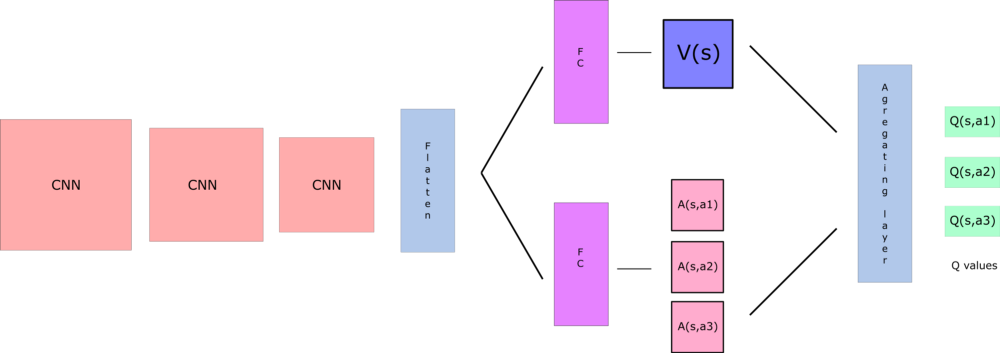
\includegraphics[width=0.72\textwidth]{img/duelingDqn.png}
	\caption{Schéma illustrant la décomposition en deux flux pour estimer séparément $A(s,a)$ et $V(s)$ \cite[]{freecodecamp}}
\end{figure}
En séparant cette estimation, notre réseau de neurones peut apprendre quel état a de la valeur sans apprendre l'effet de chaque action à chaque état. Ceci est particulièrement utile pour des états où les actions qui y sont liés ne provoquent pas un changement conséquent de l'environnement. Ceci accélère encore l'apprentissage du modèle vu qu'on a moins de combinaisons d'états-actions à calculer.
\subsubsection{Prioritized experience replay}
Le Prioritized experience replay (PER) a été introduit en 2015, l'idée est que certaines expériences peuvent être plus importants que d'autres pour notre entraînement mais peuvent survenir rarement.

Vu que l'échantillonage de la mémoire se fait d'une façon aléatoire uniforme, ces expériences importantes qui surviennent pas souvent n'ont pas beaucoup de chances d'êtres sélectionnés.

L'idée du PER est de changer la distribution aléatoire de l'échantillonage de la mémoire en utilisant un critère définissant une priorité pour chaque tuple d'expérience stocké.

Les expériences qui devraient être priorisées sont celles où il y a une grande différence entre la prédiction de la Q-value et la Q-target, ce qui veut dire qu'on a plus à apprendre de cette expérience vu qu'elle a donné une estimation de la Q-value qui était plus fausse que d'habitude.
\section{Rainbow}
Dernièrement (octobre 2017) a été développé et testé par DeepMind \cite[]{Rainbow} un algorithme s'appelant "rainbow".
\begin{figure}[H]
	\centering
	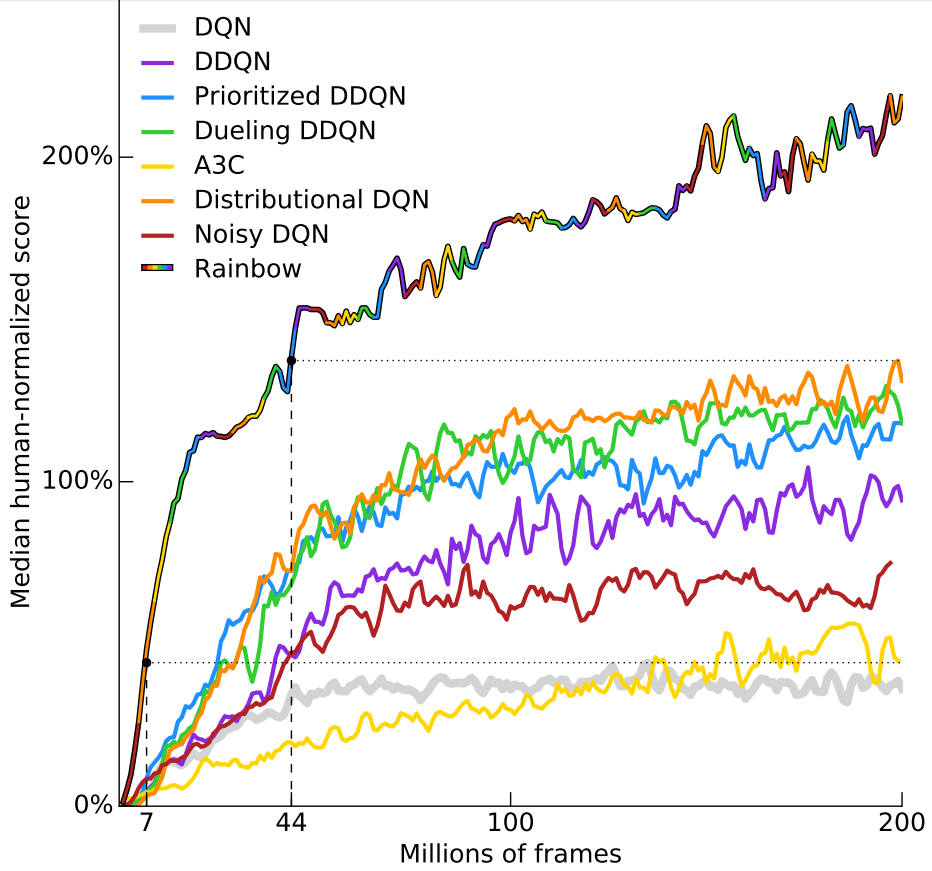
\includegraphics[width=0.45\textwidth]{img/rainbow.png}
	\caption{Graphique montrant le résultat des tests pour des scénarios où l'agent joue à des jeux Atari, le score est mesuré et comparé à un score qu'un humain aurait fait en moyenne \cite[]{Rainbow}}
\end{figure}

La figure 1.9 montre d'où vient le nom "rainbow" : chaque couleur représente une façon de faire du DQN, et "rainbow" est la combinaison de toutes ces méthodes ce qui donne un arc en ciel.

On peut remarquer que rainbow intègre toutes les techniques améliorant le deep Q-Learning expliqué dans la section précédente, et bien plus encore.

Selon la figure 1.9 les résultats issu de l'utilisation de cet algorithme dépassent largement tous les autres dans le cas des jeux Atari, c'est pourquoi il a été jugé intéressant d'essayer un framework implémentant cet algorithme dans le cadre de ce projet, les résultats issu de cet essai sont expliqués dans le chapitre suivant.

\chapter{Analyse}
\thispagestyle{headings}

\section{Comparaison de frameworks de Reinforcement Learning}
La première phase du projet hormis la prise en main des algorithmes de Reinforcement Learning, a été de d'explorer et de comparer deux frameworks facilitant la mise en place d'algorithmes de Reinforcement Learning pour pouvoir les appliquer à un scénario donné.

Pour la comparaison a été choisi le jeu-vidéo Doom dont l'interfaçage avec un agent RL a été rendu possible grâce à ViZDoom \cite[] {Kempka2016ViZDoom}

Ce choix a été fait car la seule façon de percevoir l'environnement de Doom pour un agent est d'analyser les pixels à l'écran, ce qui est que possible avec les techniques de Deep Q Learning et c'était donc une façon de tester à pleine puissance les frameworks retenus.

Le scénario utilisé pour la comparaison faisait partie de ceux fournis par ViZDoom \cite[]{vizDoomScenario}, s'appellant "defend the line" il consistait en un niveau de jeu conçu spécialement pour tester la performance d'un agent à survivre le plus longtemps dans un environnement où le but était de tirer sur des ennemis apparaissant en face de lui.

Les actions que pouvait entreprendre l'agent étaient les suivants:
\begin{itemize}
	\item Tourner à gauche
	\item Tourner à droite
	\item Tirer droit devant avec un pistolet
\end{itemize}
Les ennemis apparaissent à des positions donnés au début de la partie, et à chaque fois qu'un ennemi meurt il réapparaît avec plus de points de vie qu'avant (à chaque réapparition il faut une balle de plus pour le tuer que la fois d'avant)

La fonction de récompense était celle proposée par défaut dans un premier temps: +1 par ennemi tué et -1 à la mort de l'agent. Cette fonction était utilisée pour comparer différents frameworks avec le même algorithme \hyperref[sec:table22]{(Table 2.2)}.

Dans un second temps, après inspiration venant de VizDoom-Keras-rl \cite[]{vizDoomkeras-rl}, il a été jugé intéressant de faire baisser la récompense de 0.1 à chaque fois que l'agent tirait avec son arme et à chaque fois qu'il perdait de la vie. Ceci pourrait lui apprendre à économiser les munition et éviter de se faire toucher par les ennemis. Cette fonction était utilisée pour les résultats de la \hyperref[sec:table23]{Table 2.3}.
\subsection{Critères de comparaison}
\subsubsection*{Caractéristiques du framework et son évaluation}
La présence ou non des éléments suivants:
\begin{itemize}
	\item Double DQN
	\item Dueling DQN
	\item PER (prioritized experience replay)
	\item Fixed Q-target
	\item Rainbow
\end{itemize}
L'évaluation des points suivants:
\begin{itemize}
	\item Facilité d'adaptation
	\item Facilité d'utilisation
	\item Facilité d'installation
	\item Facilité d'interfaçage avec un environnement personnalisé
	\item Qualité de la documentation
\end{itemize}

Et deux critères "pratiques"
\begin{itemize}
	\item Systèmes d'exploitations supportés
	\item Dernière mise à jour sur github (au moment de la comparaison)
\end{itemize}
\subsubsection*{Mesures quantifiables pour un scénario donné}
\begin{itemize}
	\item Temps d'apprentissage pour 750 épisodes
	\item Score moyen sur 100 épisodes de test
\end{itemize}
Le nombre de 750 épisodes d'apprentissage vient du fait que c'est à partir de là que la version "sans framework" \cite[]{sansFramework} du algorithme donnait des résultats satisfaisants, c'est à dire que l'agent avait développé un comportement lui permettant de survivre dans le scénario en visant les ennemis explicitement avant de leurs tirer dessus.


Le nombre de 100 épisodes de test a été jugé suffisant pour que l'influence de facteurs aléatoires ne soit pas significative.
\newpage
\subsection{Démarche de test}
Afin d'avoir la comparaison la plus juste possible entre les frameworks, il a fallu dans un premier temps comparer les résultats pour un même algorithme donné et avec les hyperparamètres se rapprochant le plus possible.

Les hyperparamètres partagés utilisés étaient les suivants:
\begin{itemize}
\item Algorithme: dans un premier temps, DQN sans améliorations
\item Fonction de score: décrite plus haut
\item Nombre de frames empilés: 4
\item Taille image originale: 320x240
\item Taille image redimensionné : 78x51
\item Learning rate: 0.00025
\item Nombre d'épisodes d'entraînement: 750
\item Taille d'échantillon issus de la mémoire (batch size) : 64
\item Epsilon variant de 1 à 0.01 avec un taux de décroissance exponentielle à 0.00005
\item Gamma (discounting rate): 0.95
\item Taille de la mémoire : 50000
\item Nombre de step d'échauffement (pour remplir la mémoire avec des échantillons aléatoires): 50000
\item Nombre d'épisodes de test: 100 
\item Réseau de neurones: 
\begin{enumerate}
	\item 4 images empilées servent à nourrir le réseau
	\item Ils passent par 3 couches de convolution
	\item Ensuite on aplatit
	\item 2 couches entièrement connectées
	\item En sortie, une Q-Value pour chaque action
\end{enumerate}
\end{itemize}

Dans un second temps, le but était de trouver le meilleur algorithme proposé par les deux frameworks retenus, donc la plupart des hyperparamètres ont été gardés (le réseau de neurones change évidemment si on utilise le double DQN par exemple), et certains hyperparamètres ont été ajoutés étant spécifique à des algorithmes.
\section{Choix de framework de Reinforcement Learning}
Les frameworks à comparer retenus ont été les suivants:
\begin{itemize}
	\item keras-rl: \link{https://github.com/keras-rl/keras-rl}
	\item dopamine: \link{https://github.com/google/dopamine}
\end{itemize}
De plus, les résultats ont été comparés avec une solution sans framework \cite[]{sansFramework}

\begin{table}[H]
	\centering
			
	\begin{tabular}{|l|l|l|}
		\hline
		                                          & \thead{dopamine}                  & \thead{keras-rl} \\ \hline
		Double DQN                                & Oui                               & Oui              \\ \hline
		Dueling DQN                               & Non                               & Oui              \\ \hline
		PER                                       & Oui                               & \makecell[l]{Oui \\(branche github: keras-rl-v0.4.2)} \\ \hline
		Fixed Q-target                            & Oui                               & Oui              \\ \hline
		Rainbow                                   & Oui                               & Non              \\ \hline
		Os supportés                             & \makecell[l]{Mac, Linux, (Windows\\si on n'utilise pas atari-py)}            & Windows, Mac, Linux                                      \\ \hline
		Dernière mise à jour du code sur github & 21.11.18                          & 06.11.18         \\ \hline
	\end{tabular}
	\caption{Comparaison de critères généraux concernant les frameworks}
\end{table}
Concernant les mises à jours du code sur github:
\begin{itemize}
	\item dopamine est mis à jour plus régulièrement mais il est assez récent sorti en Août 2018) donc beaucoup de mises à jour corrigent des bugs et le rendent plus modulaire
	\item keras-rl est mis à jour plus rarement mais il est déjà mature ( sorti en Juillet 2016) donc il a moins de bugs et plus de modularité a été ajouté depuis le temps qu'il a été mis en ligne pour la première fois
\end{itemize}

Il est à noter que l'implémentation de l'algorithme rainbow dans dopamine diffère de celle du papier scientifique publié par Google DeepMind \cite[]{Rainbow}

dopamine n'implémente que les éléments suivants en plus de l'algorithme DQN de base:
\begin{itemize}
	\item Double Q Learning (pas mis sur le README du projet, mais présent et implémenté dans le code)
	\item n-step Bellman updates (fixed Q-target)
	\item Prioritized experience replay
	\item Distributional reinforcement learning (C51)
\end{itemize}
Dans le papier scientifique, les éléments suivants étaient présent mais ne sont pas implémentés dans dopamine:
\begin{itemize}
	\item Dueling networks
	\item Noisy nets
\end{itemize}

\subsubsection*{Evaluation de keras-rl}
Facilité d'adaptation
\begin{itemize}
	\item (moyen) Dans \lstinline{dqn.fit} on peut définir qu'une limite en steps et pas une limite en épisodes par défaut mais c'est facilement modifiable
	\item (moyen) L'implémentation du PER a dû être récupérée dans une branche séparé sur github car le PER n'est pas supporté dans la version de la branche master
	\item (bien) Système de callback prévu pour appeler une certaine fonction à des étapes importantes de l'entraînement ou de l'évaluation: par exemple au début de l'entraînement, à la fin de chaque épisode, à la fin de l'entraînement
	\item (bien) Classes abstraites prévues pour interfacer les agents disponibles dans le framework avec un environnement personnalisé et pour écrire ses propres fonctions callback pour faire du logging
\end{itemize}

Facilité d'utilisation
\begin{itemize}
	\item (bien) Si on se base sur les exemples fournis
	\item (bien) Les réseaux de neurones utilisent keras, qui est plus facile à utiliser que \lstinline{tf.slim}
\end{itemize}

Facilité d'installation
\begin{itemize}
	\item (bien) Pas de soucis particuliers
\end{itemize}

Facilité d'interfaçage avec environnement existant
\begin{itemize}
	\item (bien) L'architecture le permet facilement
\end{itemize}

Qualité de la documentation
\begin{itemize}
	\item (moyen) la documentation \cite[]{rlDoc} contient quelques "write me" mais les points importants (quel module sert à quoi et comment) sont bien expliqués, quelques fois se plonger dans le code source était nécessaire mais il est bien commenté et l'utilité de diverses parties du code est claire, de plus on peut facilement se baser sur les quelques exemples disponibles sur github pour bien comprendre le fonctionnement du framework
\end{itemize}

\subsubsection*{Evaluation de dopamine}

Facilité d'adaptation
\begin{itemize}
	\item (moyen) Architecture modulaire: \textbf{agent}, \textbf{environnement}, "\textbf{runner}" (gère ce qu'il faut faire entre les épisodes par exemple)
	\item (bien) Dans \lstinline{Runner.run_one_phase} on peut définir qu'une limite en steps et pas une limite en épisodes par défaut (ce qui est suffisant selon les besoins d'un scénario, mais dans mon cas la condition d'arrêt d'un entraînement était un nombre d'épisodes), mais c'est facilement modifiable
\end{itemize}

Facilité d'utilisation
\begin{itemize}
	\item (bien) Si on veut utiliser l'environnement atari fourni par défaut on n'a rien à faire
	\item (bien) Si on veut modifier les réseaux de neurones, dopamine utilise \lstinline{tf.slim} qui offre une couche d'abstraction par dessus tensorflow donc c'est plus facile qu'avec tensorflow de base
\end{itemize}

Facilité d'installation
\begin{itemize}
	\item (bien) Pas de soucis particuliers, sauf si on veut utiliser  sur windows l'environnement atari fourni par défaut (il n'y a pas de version pour windows du module atari-py)
\end{itemize}

Facilité d'interfaçage avec environnement existant
\begin{itemize}
	\item (moyen) L'architecture le permet facilement même s'il n'y a pas de documentation fait pour, il faut étudier le code source pour comprendre comment faire
\end{itemize}

Qualité de la documentation
\begin{itemize}
	\item (bien) Les points importants sont bien expliqués \cite[]{dopamineDoc} (organisation et utilité des modules du framework), il y a peu d'exemples mais les plus importants sont là (comment créer un agent personnalisé, visualiser résultats avec tensorboard)
\end{itemize}

\subsection{Résultats des tests}

\begin{table}[H]
	\label{sec:table22}
	\centering
			
	\begin{tabular}{|l|l|l|l|}
		\hline
		                                         & \thead{dopamine} & \thead{keras-rl} & \thead{sans framework} \\ \hline
		Temps d'apprentissage pour 750 épisodes & 2h               & 2h               & 9h19                   \\ \hline
		Score moyen sur 100 épisodes de test    & 10.84            & 13.97            & 3.19                   \\ \hline
	\end{tabular}
	\caption{Comparaison entre frameworks pour un scénario de test et algorithme donné (DQN sans améliorations avec fonction de score par défaut sur le scénario "defend the line")}
\end{table}

\begin{table}[H]
	\label{sec:table23}
	\centering
		
	\begin{tabular}{|l|l|l|l|l|}
		\hline
		                                         & \thead{dopamine\\implicit quantile} & \thead{dopamine\\rainbow} & \thead{keras-rl\\dqn+} & \thead{keras-rql\\dqn} \\ \hline
		Temps d'apprentissage pour 750 épisodes & 53 m            & 48 m & 3h52   & 2h7  \\ \hline
		Score moyen sur 100 épisodes de test    & 5.8             & 6.25 & 16.837 & 4.04 \\ \hline
	\end{tabular}
	\caption{Comparaison entre frameworks et algorithmes pour un scénario de test donné, avec une fonction de score différente que celle utilisée dans le tableau précédent (dqn+ représente l'algorithme dqn avec toutes les améliorations activables dans keras-rl)}
	
	
\end{table}

L'agent implémentant implicit quantile hérite de celui qui implémente rainbow donc il est sensé ajouter plus d'améliorations à l'algorithme.

Beaucoup de variations des hyperparamètres sur les deux algorithmes disponible dans dopamine n'ont pas donné de différences significatives aux scores.

Plusieurs entraînement ont été effectués, et bien que le score d'évaluation varie d'une fois à l'autre, l'ordre de grandeur de différence entre dopamine et keras-rl reste le même.

\subsubsection*{Conclusion des tests}
Étonnamment, c'est keras-rl qui a largement de meilleurs scores avec son meilleur algorithme DQN par rapport aux deux implémentations de l'algorithme rainbow de dopamine.

Par contre au niveau du temps que prends un entraînement pour le même nombre d'épisodes, les algorithmes implémentés par dopamine (rainbow et dérivées) sont beaucoup plus rapides.

Dans les évaluations des agents entraînés avec dopamine a été observé une certaine "paresse" de l'agent, c'est à dire qu'il se contenait au bout d'un moment (une fois que l'epsilon a fini de diminuer) de ne plus tourner ni à gauche ni à droite et il tirait en face de lui même sans ennemis devant mais il finissait par en toucher ceux qui passaient devant lui.

Par contre l'agent entraîné avec keras-rl se tournait en direction des ennemis quand ils apparaissaient et leurs tirait dessus de façon ciblé, ce qui augmentait sa durée de survie et donc son score, ce qui prouve un certain apprentissage permettant de faire le lien entre les ennemis apparaissant sur l'écran et l'action de leur tirer dessus pour augmenter son score

La seule chose que l'algorithme utilisé par keras-rl avait de plus que dopamine était le dueling network, mais après des tests supplémentaires où cette fonctionnalité était désactivée, keras-rl était quand même meilleur, avec un écart moins important.

Peut être que l'implémentation de dopamine visait à améliorer les performances dans le cadre des jeux Atari, utilisés pour mesurer la performance de leur algorithme dans leur papier scientifique et sur lesquels le framework repose par défaut. Ce qui améliorait les résultats dans les jeux Atari n'est peut être pas valable dans le cadre d'un scénario sur Doom, d'où cette surprise et différence au niveau des scores obtenus.

Plus tard pendant la phase d'implémentation quand le sujet d'étude était le scénario FlappyBird, de nouveaux tests ont été menés pour voir si dopamine serait plus efficace dans un environnement non visuel. L'ordre de grandeur de la différence des scores entre dopamine et keras-rl était le même que pour Doom et donc la conclusion des paragraphes précédents reste inchangé.

\subsection{Motivation du choix}
Au niveau des critères relatifs à l'évaluation (facilité d'utilisation, documentation etc.), les deux frameworks se valent. keras-rl a une certaine maturité par rapport à dopamine ce qui le rends moins risqué au niveau de potentiels bugs.

Il a été jugé que le critère du temps que prends un entraînement est moins important que le score obtenu, donc le choix a été fait d'utiliser keras-rl et non pas dopamine pour la suite de ce travail.
\chapter{Conception}
\thispagestyle{headings}

\section{Choix des critères de mesure}
Au début, c'est le score qui a été choisi pour comparer l'efficacité d'une configuration de hyperparamètres par rapport à une autre.

Sauf que ce choix avait un problème: vu que la fonction de score fait partie des hyperparamètres, quand elle est changée, la comparaison avec les configurations précédentes n'est plus pertinente.

La solution finale a été de comparer le nombre de frames que l'agent survit chaque épisode, vu que les deux scénarios consistent à survivre le plus longtemps possible dans un niveau, cette mesure est un indicateur qui est indépendant des hyperparamètres et qui permet justement de comparer efficacement une configuration à une autre.
\section{Choix des jeux pour tester les algorithmes}
\subsection{Doom}
La décision a été prise de continuer d'utiliser Doom, pour avoir un environnement représenté par des pixels. Ceci permettra d'utiliser le plein potentiel du framework, car c'est un problème qui est difficile pour un agent à apprendre avec des techniques conventionnelles à cause du nombre de données qu'engendrent ces pixels pour représenter un état.

Il est à noter qu'en plus des pixels, l'environnement nous fourni diverses variables à chaque step du jeu, voici celles qui étaient utilisés notamment pour la fonction de score:
\begin{itemize}
\item Points de vie de l'agent
\item Munitions de l'arme actuelle
\item Nombre de fois que notre arme a touché un ennemi
\end{itemize}
\subsubsection{Choix du scénario doom}
Le choix a été pris de continuer avec le même scénario que celui utilisé pour comparer les différents frameworks dans le chapitre précédent (defend the line), car c'était un problème relativement simple où l'optimisation des hyperparamètres tels que la fonction de récompense serait le plus aisé.

Le scénario se compose d'un fichier .wad qui contient la description du niveau: l'agencement en 3d du niveau et les scripts qui décrivent la logique (fonction de récompense par défaut et faire apparaître les ennemis au début du niveau et ensuite quand on les tue en augmentant leurs points de vie)
\subsection{Flappy Bird}
L'interaction entre flappy bird et le jeu était rendu possible grâce à PLE (PyGame Learning Environment) \cite[]{tasfi2016PLE}

PLE propose pour chaque scénario (jeux) une ou deux façons de récupérer les informations relatives à l'environnement: soit les pixels à l'écran soit dans un dictionnaire contenant diverses variables décrivant l'environnement.

C'est pour la présence de cette dernière option que Flappy Bird a été choisi, pour avoir un exemple d'environnement décrit avec un petit nombre de variables, mais qui suffit amplement pour décrire cet environnement dans ce cas.

Les actions que pouvait entreprendre l'agent à chaque frame étaient la possibilité de sauter ou ne rien faire.
\section{Architecture logicielle}
\begin{figure}[H]
	\centering
	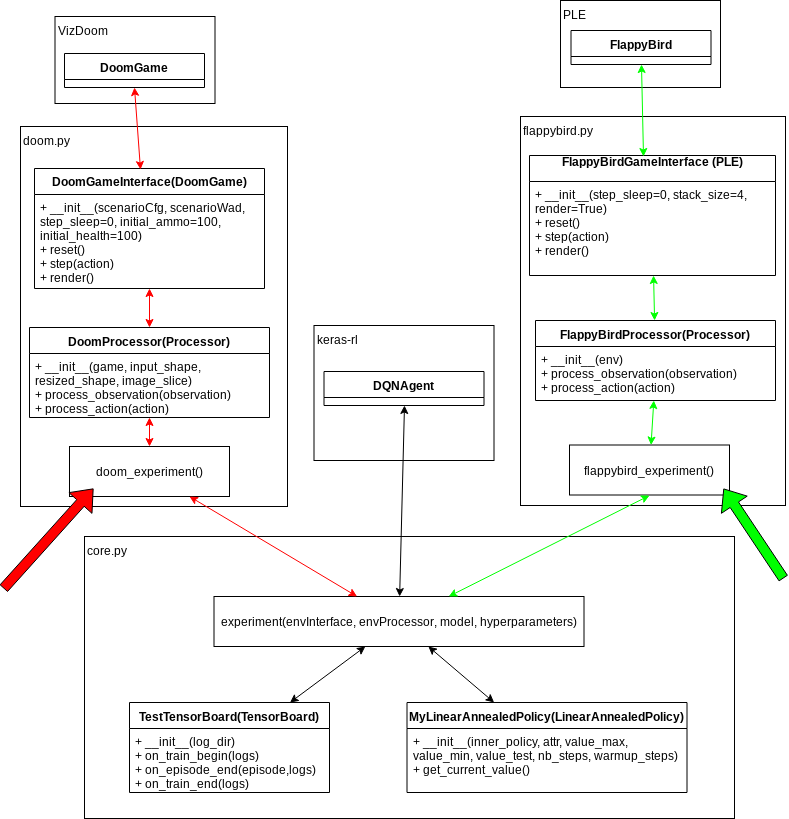
\includegraphics[width=0.99\textwidth]{img/classes.png}
	\caption{Les grosses flèches remplies représentent le points d'entrée des programmes (rouge pour Doom et vert pour FlappyBird)\hspace{\textwidth}Les Les flèches fines ne sont pas de l'héritage au sens UML mais représentent l'interaction entre les divers composants\hspace{\textwidth}Les flèches noires sont communes à Doom et Flappybird, les flèches rouges ne concernent que Doom et les flèches vertes ne concernent que FlappyBird}
\end{figure}

\chapter{Implémentation}
\thispagestyle{headings}

% \begin{lstlisting}
% 	#Test latex
% 	def foo(a,b):
% 		return a-b
% \end{lstlisting}

% \begin{algorithm}[H]
%   \KwData{this text}
%   \KwResult{how to write algorithm with \LaTeX2e }
%   initialization\;
%   \While{not at end of this document}{
%    read current\;
%    \eIf{understand}{
%     go to next section\;
%     current section becomes this one\;
%     }{
%     go back to the beginning of current section\;
%    }
%   }
%   \caption{How to write algorithms}
%  \end{algorithm}

\section{Description de l'environnement de développement}
%Tableau avec versions des programmes utilisés (ViZDoom, keras-rl, tensorflow, keras), général autant pour doom que flappybird

%ViZDoom:  1.1.6
% Name: tensorflow
% Version: 1.12.0
% Name: tensorboard
% Version: 1.12.0
% Name: Keras
% Version: 2.2.4
% keras-rl: commit e94ef88 sur branche master avec per venant du commit 0e5dc94 de la branche keras-rl-v0.4.2
% ple: cpmmit ba6ac84 sur branche master

Voici un tableau récapitulatif des différentes versions des outils utilisés dans ce projet:

\begin{table}[H]
	\resizebox{\textwidth}{!}{\begin{tabular}{|l|l|l|l|l|l|l|l|}
		\hline\thead{outil}         & \thead{ViZDoom} & \thead{tensorflow} & \thead{tensorboard} & \thead{Keras} & \thead{keras-rl}   & \thead{ple} & \thead{scikit-image}     \\
		\hline\thead{version pip}   & 1.1.6   		  & 1.12.0     & 1.12.0      & 2.2.4 &       &         & 0.14.2         \\
		\hline\thead{commit github} &                 &            &             &       & \makecell{e94ef88 (master)\\0e5dc94(keras-rl-v0.4.2)} & ba6ac84 (master) & \\
		\hline             
	\end{tabular}}
	\caption{Tableau récapitulatif des différentes versions des outils utilisés dans le projet}
\end{table}
A noter que pour keras-rl, l'implémentation du PER vient d'une autre branche que master
\section{Doom}
\subsection{Réseau de neurones}
Les données nourrissant le réseau de neurones sont un empilement de 4 images en niveau de gris recadrés et redimensionnés, les images sont fournis par l'environnement ViZDoom

\subsubsection*{Explication des étapes et couches du réseau de neurones:}
\begin{enumerate}
	\item L'image venant de Doom est déjà en niveaux de gris et a une taille de 320x240
	\item Des parties inutiles ont été coupées de l'image venant du jeu (voir figure 4.1)
	\item L'image est ensuite redimensionnée pour prendre moins de place (78x51 dans une première configuration utilisé dans le tableau résumant le réseau de neurones de la page suivante, 160x84 dans une 2ème configuration expliquée plus tard)
	\item Ceci s'applique pour 4 images pris à la suite temporellement qui sont ensuite empilés, permettant d'avoir une notion de temporalité
	\item Une première couche normalise les niveaux de gris (division par 255)
	\item Une seconde couche fait une permutation des paramètres d'entrée pour correspondre au format qu'attends keras-rl
	\item Diverses couches de convolution s'inspirant des travaux venant de VizDoomkeras-rl \cite[]{vizDoomkeras-rl}
	\item Finalement, les dernières couches servent à estimer la Q-Value pour l'état passé en entrée dans le réseau et prendre la décision d'effectuer l'action ayant la plus haute Q-Value
	\item Il est à noter que si on active de dueling network, keras-rl utilise les dernières couches du réseau de neurones qu'on lui fournit pour les "séparer" en deux flux selon l'algorithme du dueling network, et fait ensuite une agrégation des deux flux séparés, donc le modèle qu'on lui passe est fait comme s'il n'était pas prévu de faire du dueling network
\end{enumerate}
\begin{figure}[H]
	\centering
	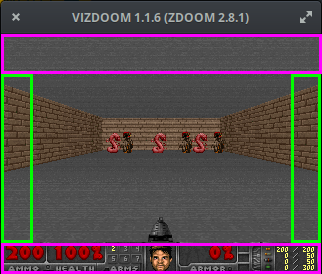
\includegraphics[width=0.5\textwidth]{img/croppedDoomFrame.png}
	\caption{En rose et vert : parties coupées pour la 1ère configuration (plus tard redimensionné en 78x51), en rose: parties coupées pour la 2ème configuration (plus tard redimensionné en 160x84)}
\end{figure}
Voici le résultat de la fonction \lstinline{model.summary()} appliqué sur le modèle passé à keras-rl:
\begin{lstlisting}
Layer (type)                 Output Shape              Param #
=================================================================
lambda_1 (Lambda)            (None, 4, 51, 78)         0
_________________________________________________________________
permute_1 (Permute)          (None, 51, 78, 4)         0
_________________________________________________________________
conv2d_1 (Conv2D)            (None, 11, 18, 32)        8224
_________________________________________________________________
activation_1 (Activation)    (None, 11, 18, 32)        0
_________________________________________________________________
conv2d_2 (Conv2D)            (None, 4, 8, 64)          32832
_________________________________________________________________
activation_2 (Activation)    (None, 4, 8, 64)          0
_________________________________________________________________
conv2d_3 (Conv2D)            (None, 1, 3, 128)         131200
_________________________________________________________________
activation_3 (Activation)    (None, 1, 3, 128)         0
_________________________________________________________________
flatten_1 (Flatten)          (None, 384)               0
_________________________________________________________________
dense_1 (Dense)              (None, 512)               197120
_________________________________________________________________
activation_4 (Activation)    (None, 512)               0
_________________________________________________________________
dense_2 (Dense)              (None, 3)                 1539
_________________________________________________________________
activation_5 (Activation)    (None, 3)                 0
=================================================================
Total params: 370,915
Trainable params: 370,915
Non-trainable params: 0
\end{lstlisting}
\subsection{Choix et optimisation des hyperparamètres}
\subsubsection*{Les hyperparamètres suivants étaient fixes tout du long}
\begin{itemize}
\item Nombre de frames empilés: 4
\item Taille de l'image de sortie du jeu: 320x240
\item Encodage de couleur des pixels: valeurs de gris
\item Batch size (taille de l'échantillon issu de la mémoire): 64
\item Max tau (fréquence de mise à jour du réseau cible en nombre de pas, utilisé pour le fixed Q-targets): 10000
\item Nombre de pas d'échauffement (remplissage de la mémoire d'actions aléatoires pour avoir assez d'échantillons au début) : 50000
\item Alpha (learning rate): 0.00025
\item Gamma (discount rate): 0.95
\item Epsilon au début de l'entraînement: 1
\item Epsilon à la fin de l'entraînement: 0.01
\item Nombre de pas pendant décroissance d'epsilon: 80000
\item Epsilon utilisé pendant la phase d'évaluation: 0.001
\item Nombre d'épisodes de test: 100
\end{itemize}
\subsubsection*{Hyperparamètres qui ont évolué et qui ont subi des optimisations}
\begin{itemize}
\item Recadrage de l'image venant de l'environnement
\begin{itemize}
	\item D'abord l'image était coupée de 40 pixels en haut pour ne pas prendre en compte le plafond qui n'apportait pas d'informations utiles, 32 pixels en bas pour ne pas prendre en compte l'interface du jeu, 30 pixels à droite et à gauche
	\item Finalement, il a été constaté que les pixels latéraux coupés empêchaient l'agent de voir les ennemis apparaissant du côté droite quand il visait l'ennemis tout à gauche, donc une configuration explorée était de ne pas couper ces pixels. Par contre si on veut avoir un contrôle plus fin sur la taille de l'image redimensionné tout en gardant le même ratio entre l'image recadrée et redimensionnée, il pourrait être judicieux de couper quelques pixels afin que le plus grand diviseur commun soit maximal entre le nombre de pixels vertical et horizontal de l'image recadrée (Par exemple si on coupe 40 pixels en haut, 32 en bas, et 6 à gauche et droite on a une résolution de 308x168 et le plus grand diviseur commun entre ces deux nombre est 28, donc on peut avoir n'importe quelle résolution qui soit un multiple de 11x6 tout en gardant le même ratio entre largeur et hauteur)
\end{itemize}
\item Taille de l'image redimensionné nourrissant le réseau de neurones
\begin{itemize}
	\item Avec la première configuration de recadrage: 78x51, avec celle-ci l'agent avait périodiquement des comportements inadéquats où il se tournait face au mur ou à un coin au bout d'un moment et se faisait tuer, une hypothèse était que la résolution de l'image redimensionné était trop basse et empêchait l'agent de percevoir correctement l'environnement dans certains cas
	\item Avec le seconde configuration de recadrage: 160x84, les comportements inadéquats de l'agent avaient disparu et les résultats se sont améliorés, mais le temps d'entraînement est devenu extrêmement grand (24h pour 500 épisodes alors qu'avec la configuration d'avant il lui fallait 4h pour 750 épisodes)
\end{itemize}
\item Fonction de décroissance d'epsilon
\begin{itemize}
	\item D'abord, la fonction de décroissance était une exponentielle négative
	\item Finalement la fonction de décroissance était linéaire, cette dernière semblait donner de meilleurs résultats
\end{itemize}
\item Fonction de score (expliqué dans la prochaine section)
\item Taille de la mémoire: quelques changement ont été tentés, mais n'ont pas influencé de façon significative les résultats, la dernière taille retenue était 250000 frames 
\item Utilisation du dueling network: sa présence ou non n'avait pas beaucoup d'impact sur le résultat (même si avec, le résultat était mieux), d'ailleurs à partir d'un moment du projet, la booléen l'activant a été oublié d'être remis à vrai, ce qui n'a pas empêché d'avoir des résultats convaincants par la suite (et ce qui importait dans l'exploration était la différence sur le score induite par un seul hyperparamètre à la fois, donc les conclusions tirés de la modification des autres hyperparamètres restent quand même cohérents)
\item Nombre d'épisodes d'entraînement: avec un bon choix des hyperparamètres précédents, on pouvait se permettre de réduire le nombre d'épisodes d'entraînement pour avoir de bons résultats
\end{itemize}
\subsection{Fonction de score}
Par défaut, le scénario donne +1 pour chaque ennemi tué et -1 quand l'agent meurt.

Ensuite, a été ajouté un score de -0.1 pour chaque balle tirée et à chaque fois que l'agent se fait toucher pour les mêmes raisons qu'expliqué dans le chapitre concernant la comparaison de keras-rl et dopamine, c'est à dire pour encourager l'agent à économiser ses munitions et éviter de se faire toucher.

Finalement, vu les spécificités du scénario qui font en sorte que les ennemis réapparaissent avec plus de points de vie qu'avant après s'être fait tué, quand l'agent leurs tire dessus sans les tuer cela ne lui apporte aucune récompense donc il aura peut être moins tendance à continuer de leurs tirer dessus vu que la récompense immédiate est moindre.

Pour pallier à cela, la fonction de score a été modifiée de sorte à ce que l'agent reçoit une recompense de +1 à chaque fois qu'il tire et touche un ennemi, qu'il le tue ou pas.

Résumé:
\begin{enumerate}
\item +1 par ennemi tué par l'agent
\item +1 par ennemi touché par l'agent
\item -0.1 par balle tirée par l'agent
\item -0.1 par perte de vie de l'agent
\item -1 quand l'agent meurt
\end{enumerate}
L'amélioration de la fonction de score avait significativement amélioré les résultats, surtout la durée de vie de l'agent
\subsection{Résultats}
\begin{figure}[H]
	\centering
	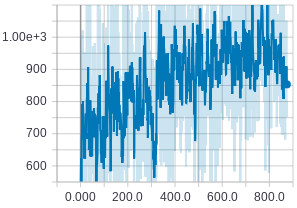
\includegraphics[width=0.32\textwidth]{img/doom_78x51.png}
	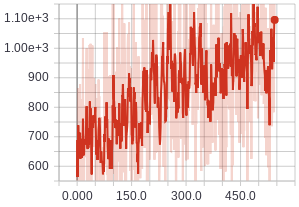
\includegraphics[width=0.32\textwidth]{img/doom_160x84.png}
	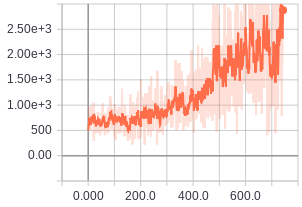
\includegraphics[width=0.32\textwidth]{img/doom_oneshotkill.png}
	\caption{Axe x: numéro de l'épisode, axe y: nombre de steps survécu pendant cet épisode\hspace{\textwidth}A gauche: version avec la taille de l'image d'entrée du réseau de neurones à 78x51\hspace{\textwidth}Milieu: l'image d'entrée est de dimension 160x84\hspace{\textwidth}A Droite: les ennemis meurent en un tir (l'image d'entrée est de dimension 78x51)}
\end{figure}

Au travers de différentes phases d'explorations, l'agent entraîné s'est de plus en plus perfectionné.

Une version modifie du .wad a été utilisée pour tester un modèle où les ennemis sont toujours tuables avec un tir, et l'agent survit jusqu'à ce qu'il n'a plus de munitions (il en a 200 au début), ce qui est une façon de prouver l'efficacité du modèle entraîné.

Avec seulement les pixels à l'écran et sans les variables fourni par ViZDoom, un résultat autant bien n'aurait pas pu être possible autant facilement, il aurait fallu analyser les pixels venant de l'interface du jeu pour récupérer le nombre de munitions et les points de vie. Pour ce qui est de savoir si un ennemi est touché, il n'y a aucune information visuelle donc ceci ne serait simplement pas possible (par contre quand un ennemi meurt il y a bien une animation distinctive).
\section{FlappyBird}
\subsection{Réseau de neurones}
Les données nourrissant le réseau de neurones sont représentés par un vecteur à 8 composantes normalisé, issu d'un dictionnaire fourni par l'environment PLE qui est le suivant:
\begin{enumerate}
\item position en Y du joueur
\item vitesse du joueur
\item distance du joueur jusqu'au prochain tuyau
\item position en Y de l'ouverture supérieure du prochain tuyau
\item position en Y de l'ouverture inférieure du prochain tuyau
\item distance du joueur jusqu'au après-prochain tuyau
\item position en Y de l'ouverture supérieure du après-prochain tuyau
\item position en Y de l'ouverture inférieure du après-prochain tuyau
\end{enumerate}

L'architecture du réseau de neurones a été construite de façon empirique, notamment en lisant un guide expliquant combien de coches/neurones il faut pour les couches intermédiaires\cite[]{layerGuide}.

L'idée retenue était qu'il fallait incrémenter au début et décrémenter à la fin le nombre de neurones par étage

Voici le résultat de la fonction \lstinline{model.summary()} appliqué sur le modèle passé à keras-rl:

\begin{lstlisting}
Layer (type)                 Output Shape              Param #   
=================================================================
dense_1 (Dense)              (None, 4, 128)            1152      
_________________________________________________________________
dense_2 (Dense)              (None, 4, 256)            33024     
_________________________________________________________________
dense_3 (Dense)              (None, 4, 512)            131584    
_________________________________________________________________
dense_4 (Dense)              (None, 4, 256)            131328    
_________________________________________________________________
dense_5 (Dense)              (None, 4, 128)            32896     
_________________________________________________________________
flatten_1 (Flatten)          (None, 512)               0         
_________________________________________________________________
dense_6 (Dense)              (None, 2)                 1026      
=================================================================
Total params: 331,010
Trainable params: 331,010
Non-trainable params: 0
\end{lstlisting}
\newpage
\subsection{Choix et optimisation des hyperparamètres}
\subsubsection*{Les hyperparamètres suivants étaient fixes tout du long}
\begin{itemize}
	\item Nombre d'empilement de l'entrée: 4
	\item Taille de la mémoire: 1000000
	\item Nombre de pas d'échauffement: 100000
	\item Présence du dueling network
	\item Nombre d'épisodes: 15000
	\item Taille d'échantillon pris dans la mémoire : 32
	\item Nombre d'épisodes de test: 100
	\item tau maximal (fréquence de mise à jour du réseau cible): 10000
	\item Alpha (learning rate) : 0.01
	\item Gamma (discount rate) : 0.95
	\item Epsilon au début : 0.15 car le nombre d'actions possibles à explorer est limité (sauter ou ne pas sauter)
	\item Epsilon à la fin 0.01
	\item Epsilon pendant phase d'évaluation: 0.001
	\item Nombre de pas pendant réduction de l'epsilon: 150000
\end{itemize}
\subsubsection*{Hyperparamètres qui ont évolué et qui ont subi des optimisations}
\begin{itemize}
	\item Réseau de neurones
	\begin{itemize}
	\item Au début, le réseau de neurones a été copié d'un exemple présent dans le github de PLE, utilisé pour le jeu "Catcher", mais il a été jugé qu'il comportait trop peu de couches
	\item Finalement, le nouveau réseau de neurones utilisait le même nombre de neurones maximales que celui précédemment (512) qui constituait la couche "au milieu" du nouveau réseau et était entouré de couches qui montaient vers ce nombre avant et descendaient après (voir le tableau dans la section au dessus)
	\end{itemize}
	\item Fonction de score : expliqué dans la section suivante
\end{itemize}
\subsection{Fonction de score}
Par défaut, la fonction de score proposée par le scénario pénalise l'agent de 5 points s'il perds et le récompense d'un point par tuyau qu'il arrive à passer

Mais avec cette fonction, c'était difficile pour l'agent de corriger ses erreurs après une mort, donc il a été décidé de le récompenser même s'il meurt écrasé contre un tuyau.

Vu que le but est de passer au mieux chaque tuyau, il devrait "viser" le milieu de chaque ouverture verticale.

Grâce aux données numériques fournis de l'environnement, il a été possible de concevoir la fonction de score suivante:

\begin{algorithm}[H]
\SetKwInOut{Input}{input}
\SetKwInOut{Output}{output}
  \Input{nextPipeBottomY, nextPipeTopY, playerPositionY, height}
  \Output{reward}
  gapMiddleYPosition $\leftarrow$ (nextPipeBottomY-nextPipeTopY)/2+nextPipeTopY\;
   \eIf{playerPositionY<gapMiddleYPosition}{
	\Return  playerPositionY/gapMiddleYPosition
    }{
	trueHeight $\leftarrow$ height*0.79\;
	\Return  1-(playerPositionY-gapMiddleYPosition)/(trueHeight-gapMiddleYPosition)
   }
  
  \caption{Fonction de score incitant l'agent de viser le milieu de l'ouverture verticale entre tuyaux}
 \end{algorithm}
 \newpage
Remarques:
\begin{itemize}
\item nextPipeBottomY, nextPipeTopY, playerPositionY sont fournis par la représentation de l'environnement à chaque step, height est un attribut de l'objet représentant l'environnement
\item l'axe Y est tourné vers le bas
\item height représente la hauteur de l'image avec le sol inclus
\item trueHeight est la hauteur maximale que peut atteindre l'agent (la limite supérieure du sol)
\item le nombre 0.79 était trouvé dans le code source de l'environnement (Donc que le 79\% de la hauteur de l'image du jeu est atteignable par l'agent, le 21\% restants est le sol en bas de l'image)
\end{itemize}
\begin{figure}[H]
	\centering
	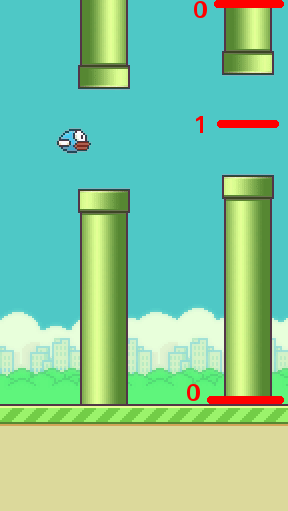
\includegraphics[width=0.35\textwidth]{img/flappyBirdScore.png}
	\caption{Représentation visuelle du score qu'aurait gagné l'agent s'il perds à cause d'une collision avec le prochain tuyau (l'intervalle en haut et en bas sont linéaires et leurs linéarité est différente pour le bas et le haut)}
\end{figure}
\newpage
\subsection{Résultats}
\begin{figure}[H]
	\centering
	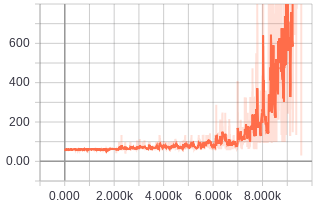
\includegraphics[width=0.4\textwidth]{img/flappybird_fit.png}
	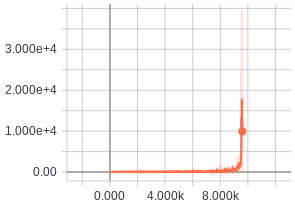
\includegraphics[width=0.4\textwidth]{img/flappybird_dezoom.png}
	\caption{Axe x: numéro de l'épisode, axe y: nombre de steps survécu pendant cet épisode\hspace{\textwidth}A gauche: Echelle du graphique permettant de voir l'évolution de la durée des épisodes\hspace{\textwidth}A Droite: Echelle du graphique permettant de voir la valeur maximale ($\sim$ 39200) et à quel point le modèle est devenu efficace}
\end{figure}

Donc avoir accès à des données numériques fourni par l'environnement est un atout considérable car on peut utiliser ces données pour diriger l'agent vers une solution souhaitée, ce qui ne serait pas possible si on n'avait accès qu'aux pixels du jeu.

Finalement on peut considérer que l'agent a "gagné" le jeu, vu qu'il arrive à faire des épisodes durant plus qu'une heure avant de perdre, ce résultat n'aurait pas pu être possible en analysant les pixels, ou alors après une durée d'entraînement beaucoup trop conséquente par rapport à la méthode actuelle.

\chapter{Conclusion}
\thispagestyle{headings}
Les modèles entraînés dans les deux jeux ont atteint des résultats très convaincants, surtout pour flappy bird.

D'autant bons résultats n'auraient pas pu être atteint avec autant d'aisance relative sans techniques de deep Q-learning pour flappy bird et n'aurait pas pu être possible du tout dans le cas de Doom.

L'hyperparamètre le plus important est sans doute la fonction de score, mais pour la définir on a besoin de variables issus d'un environnement qui étaient dans notre cas mises à disposition exprès pour être exploité dans un cadre de Reinforcement Learning. 

Mais la question qu'on pourrait se poser est: est-ce que le Reinforcement Learning serait une solution miracle pour entraîner des modèles dans des simulations et ensuite les appliquer dans la vraie vie ?

La réponse est nuancée, pour avoir des bons résultats il faut donc avoir accès à des données pas forcément mises à disposition dans n'importe quel environnement.

Dans une simulation il est relativement facile d'avoir accès à ces données, pour autant qu'on aie accès au code source de la simulation ou une API nous fournissant des données utiles.

Mais pour appliquer ensuite ce modèle entraîné dans la vraie vie, il faudrait mettre en place divers capteurs mesurant des données utiles à notre modèle, une simple caméra nous fournissant des pixels ne suffirait pas d'avoir des résultats convaincants autant facilement qu'avec les méthodes utilisées dans le cadre de ce projet.

Donc non, ce n'est pas une solution miracle car il faut un travail d'adaptation conséquent selon avec quel environnement on veut interfacer notre agent. De plus, il faudrait avoir accès aux mêmes données que celles utilisées dans l'entraînement du modèle si on voudrait l'appliquer en dehors d'un simulateur.
\subsubsection*{Apport personnel grâce au projet}
Ce projet m'a permis d'acquérir/améliorer les compétences suivantes, en plus de ce qui touche au Reinforcement Learning:
\begin{itemize}
	\item Découverte de quelques astuces en python et de nouveaux modules comme numpy
	\item L'étude en détail et la compréhension des codes sources sur github en essayant de comprendre comment il marche (surtout pendant la phase de comparaison dopamine vs keras-rl)
	\item Tout ce qui touche aux réseaux de neurones en général, CNN, tensorflow, keras, tensorboard
	\item La mesure et l'interpretation de données d'expériences
	\item Quelques fonctionnalités et modules de LaTeX
\end{itemize}
\chapter{Annexes}
\thispagestyle{headings}
\section{Manuel d'utilisation}
\subsection*{Installation}

\begin{itemize}
	\item navigate to \lstinline{src} folder
	\item \lstinline{python3 -m venv venv_rl}
	\item \lstinline{source venv_rl/bin/activate}
	\item \lstinline{pip install -r requirements.txt}
	\item All the commands in this user guide must be executed in the $src$ folder (where $doom.py$ and $flappybird.py$ are located)
\end{itemize}

\subsection*{Tensorboard logs location}
They are located in $xxx\_saves/yyy/logs/zzz$
\begin{itemize}
	\item $xxx$ is either "doom" or "flappybird"
	\item $yyy$ is the experiment name
	\item $zzz$ is either "train" or "test$N$" with $N$ empty or a number
\end{itemize}

\subsection*{Model weights location}
they are located in $xxx\_saves/yyy/weights.h5f$
\begin{itemize}
	\item $xxx$ is either "doom" or "flappybird"
	\item $yyy$ is the experiment name
\end{itemize}
\newpage
\subsection*{Doom (doom.py)}
\subsubsection*{Command line arguments}
\raggedright
All those arguments have default values except "weights"
\begin{itemize}
\item mode: "test" "train" or "watch", if set to "watch" or "test" and no weights argument specified, it will use the last trained model (default: train)
\item weights: path to trained model weights file ($.h5f$ format) (only test and watch mode, default: none)
\item step-sleep: number of ms to sleep between each step (useful to observe for a human the agent playing, default: 0)
\item test-episodes: number of episodes to test (only test and watch mode, default: 100)
\item train-episodes: number of episodes to train (only train mode, default: 780)
\item warmup-steps: number of steps for warmup (only train mode, default: 50000)
\item wad: path to wad file containing doom scenario (default: $doom\_scenarios/defend\_the\_line.wad$)
\item image-shape: shape of the image to be put in the neural network, 78x51 or 160x84 (default: 78x51)
\end{itemize}
\subsubsection*{How to watch interesting trained models at ~60 fps without tensorboard logging by loading weight file}
\begin{itemize}
	\item One shot ennemy kill with 160x84 image shape: 
	\item \lstinline{./doom.py --mode=watch --weights=doom_saves/160x84/weights.h5f  --step-sleep=15 --wad=doom_scenarios/defend_the_line-oneShotKill.wad --image-shape=160x84}
	\item one shot ennemy kill with 76x51 image shape (sometimes the agent last longer than in the 160x84 version and sometimes his behaviour is messy): 
	\item \lstinline{./doom.py --mode=watch --weights=doom_saves/oneShotKill/weights.h5f --step-sleep=15 --wad=doom_scenarios/defend_the_line-oneShotKill.wad --image-shape=78x51}
	\item normal scenario with 160x84 image shape: 
	\item \lstinline{./doom.py --mode=watch --weights=doom_saves/160x84/weights.h5f --step-sleep=15 --image-shape=160x84}
	\item normal scenario with 76x51 image shape: 
	\item \lstinline{./doom.py --mode=watch --weights=doom_saves/78x51/weights.h5f --step-sleep=15 --image-shape=78x51}
\end{itemize}
\subsubsection*{How to train + test a new model}
\begin{itemize}
	\item creates a new folder named $doom\_saves/\{saveFolder\}-\{x\}$ where $x$ is a number and $saveFolder$ "78x51" or "160x84"
	\item example: 78x51 image size, normal scenario, 100 train episodes, 20000 warmup steps, 20 test episodes: 
	\item \lstinline{./doom.py --mode=train --train-episodes=100 --warmup-steps=20000 --test-episodes=20 --image-shape=78x51}
\end{itemize}
\subsubsection*{Re test previously trained model (from previous example)}
\begin{itemize}
	\item creates a new folder named $doom\_saves/\{saveFolder\}/logs/test\{x\}$ folder where x is a number and saveFolder "78x51-1" for example
	\item example: re test previous trained model: 
	\item \lstinline{./doom.py --mode=test --test-episodes=20 --image-shape=78x51}
\end{itemize}
\newpage
\subsubsection*{Test a model by loading weight file and log test}
\begin{itemize}
	\item creates a new folder named $doom\_saves/\{saveFolder\}/logs/test\{x\}$ folder where x is a number and saveFolder "78x51-1" for example, the saveFolder is parsed from the weight file path (if the weight file is located at $foo/toto/tutu/weights.h5f$, saveFolder : $foo/toto/tutu$)
	\item  example: load and test previously trained model "$doom\_saves/78x51-1/weights.h5f$"
	\item \lstinline{./doom.py --mode=test --test-episodes=2 --image-shape=78x51 --weights=doom_saves/78x51-1/weights.h5f}
\end{itemize}
\subsection*{Flappy bird (flappybird.py)}
\subsubsection*{Command line arguments}
All those arguments have default values except "weights"
\begin{itemize}
\item  mode: "test" "train" or "watch", if set to "watch" or "test" and no weights argument specified, it will use the last trained model (default: train)
\item  weights: path to trained model weights file ($.h5f$ format) (only test and watch mode, default: none)
\item  step-sleep: number of ms to sleep between each step (useful to observe for a human the agent playing, default: 0)
\item  test-episodes: number of episodes to test (only test and watch mode, default: 100)
\item  train-episodes: number of episodes to train (only train mode, default: 16700)
\item  warmup-steps: number of steps for warmup (only train mode, default: 100000)
\item  render: render the graphics of the game or not, if set to "0" do not render, if set to anything else, render
\end{itemize}
\subsubsection*{How to watch interesting trained models at ~60 fps without tensorboard logging by loading weight file}
\begin{itemize}
	\item To test the model that "won" the game:
	\item \lstinline{./flappybird.py --mode=watch --step-sleep=15 --weights=flappybird_saves/best/weights.h5f}
\end{itemize}
\subsubsection*{How to train + test a new model}
\begin{itemize}
	\item creates a new folder named $flappybird\_saves/experiment-\{x\}$ where $x$ is a number, "$flappybird\_saves/experiment-1$" for example
	\item \lstinline{./flappybird.py --mode=train --test-episodes=50 --train-episodes=250 --warmup-steps=1000}
\end{itemize}
\subsubsection*{Re test previously trained model (from previous example)}
\begin{itemize}
\item creates a new folder named $flappybord\_saves/experiment-\{y\}/logs/test\{x\}$ folder where x and y are numbers, "$flappybird\_saves/experiment-1/logs/test2$" for example
\item \lstinline{./flappybird.py --mode=test --test-episodes=50}
\end{itemize}
\subsubsection*{Test a model by loading weight file and log test}
\begin{itemize}
	\item creates a new folder named $flappybird\_saves/\{saveFolder\}/logs/test\{x\}$ folder where x is a number and saveFolder : "best" for example, the saveFolder is parsed from the weight file path (if the weight file is located at $foo/toto/tutu/weights.h5f$, saveFolder : $foo/toto/tutu$)
	\item \lstinline{./flappybird.py --mode=test --weights=flappybird_saves/experiment-1/weights.h5f}
\end{itemize}

\section{Cahier des charges}
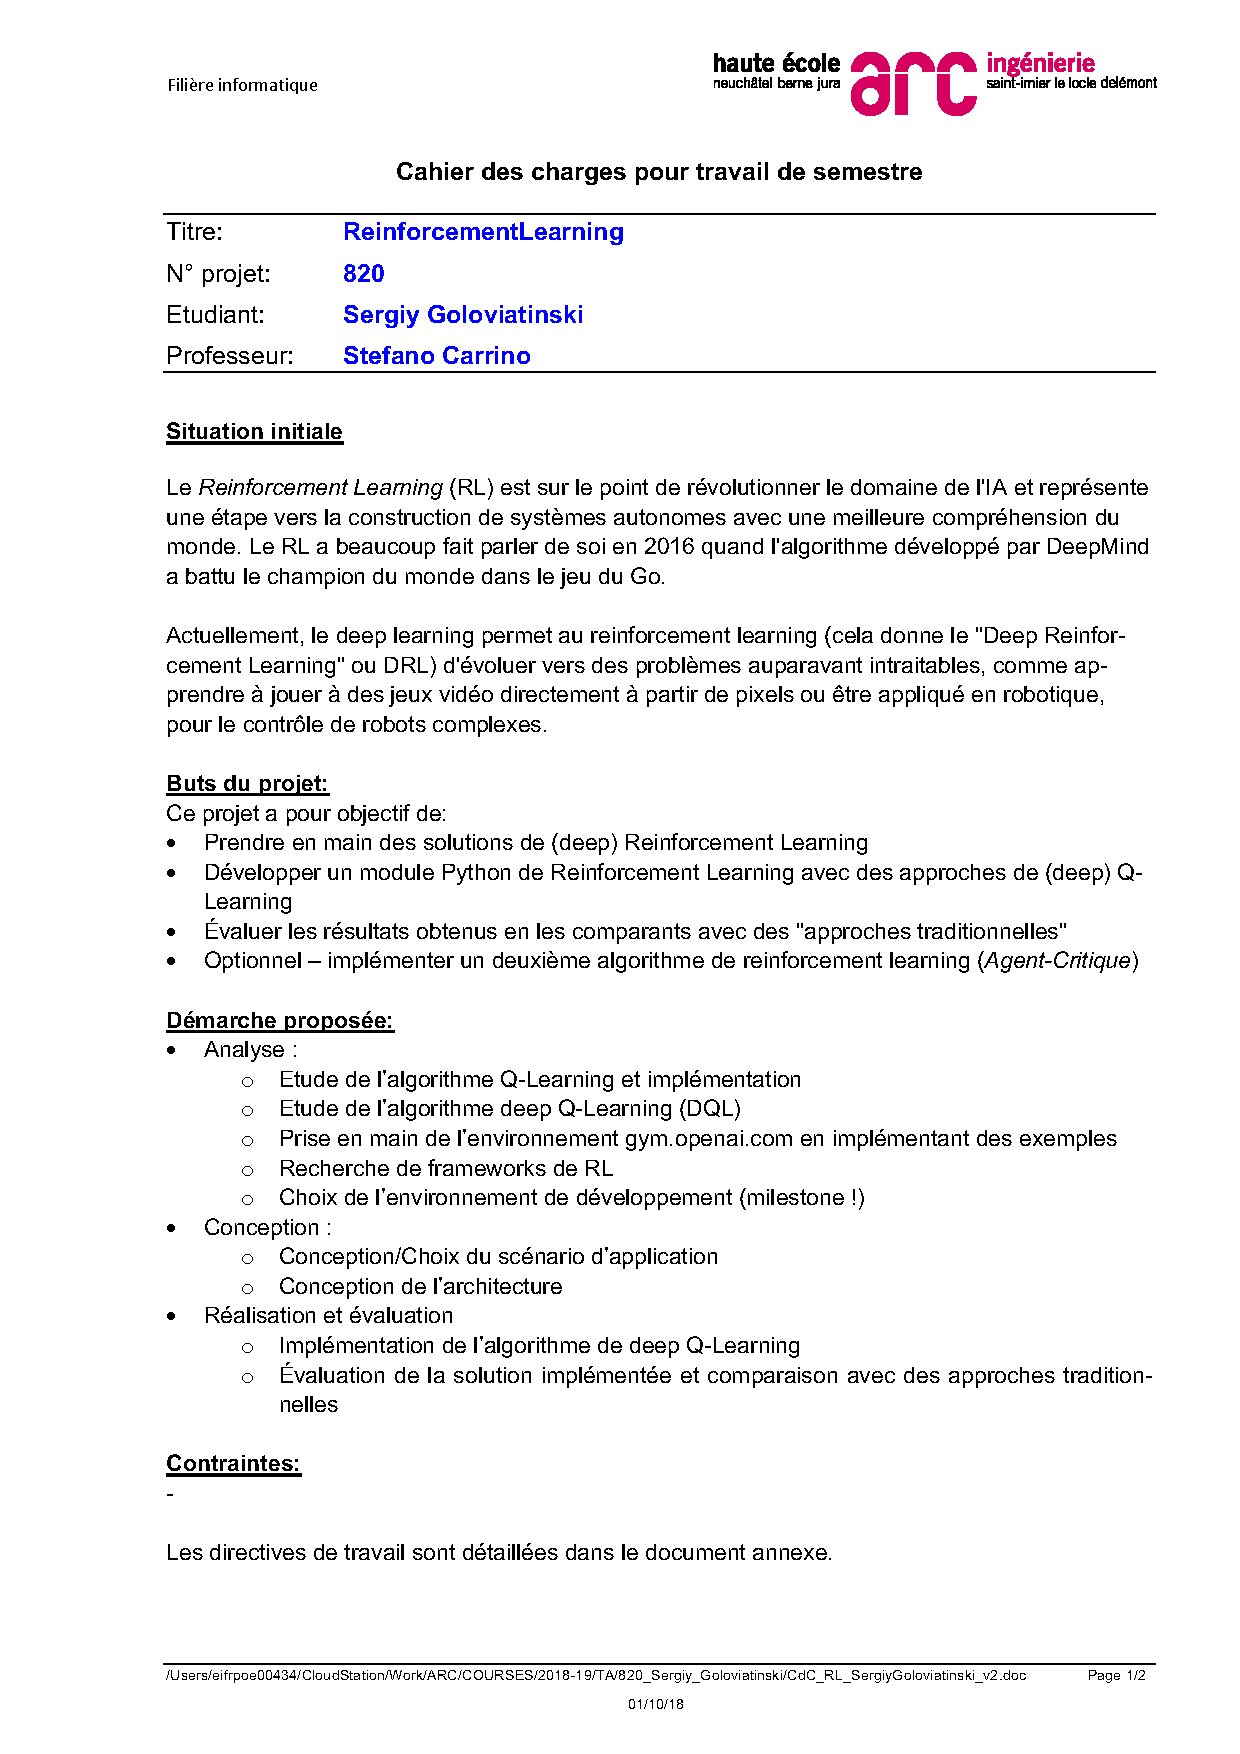
\includegraphics[
    page=1,
    width=\textwidth,
    height=0.95\textheight,
    keepaspectratio
]{res/cdc.pdf}

\section{Planning initial}
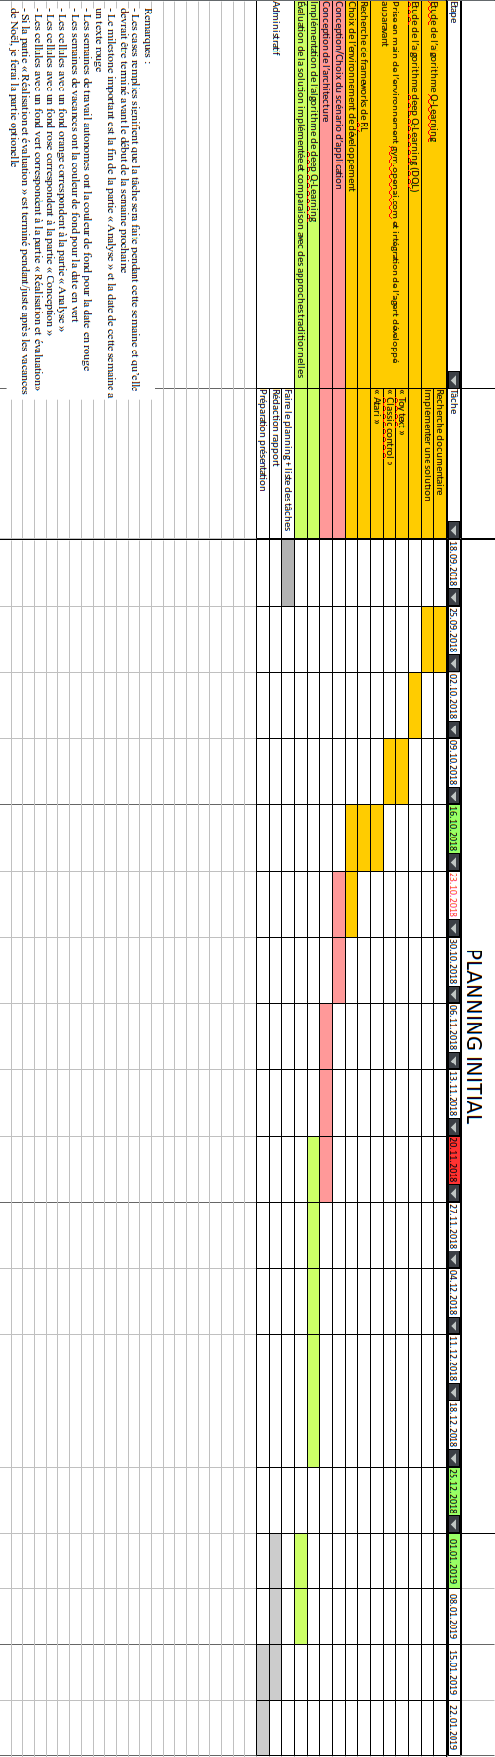
\includegraphics[
    page=1,
    width=\textwidth,
    height=0.95\textheight,
    keepaspectratio
]{res/planningInitial.pdf}
\section{Planning final}
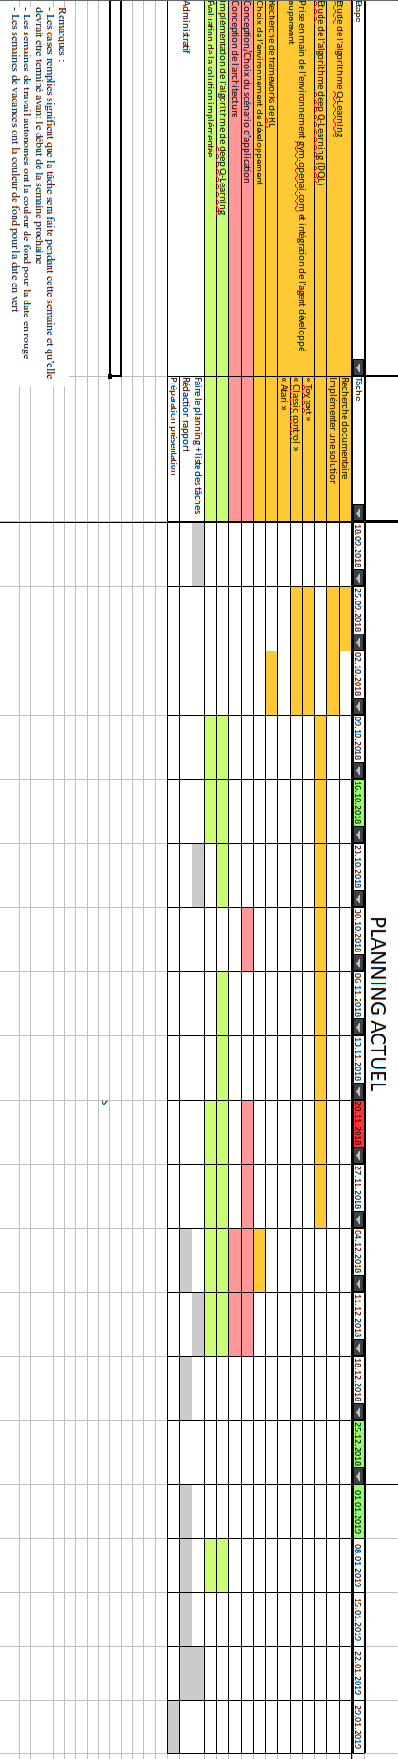
\includegraphics[
    page=1,
    width=\textwidth,
    height=0.95\textheight,
    keepaspectratio
]{res/planningActuel.pdf}
\section{Journal de laboratoire}
Total d'heures travaillées: 153h

\begin{lstlisting}
	# Semaine 15
	## 25.01.09 ~5h
	- Redaction du rapport
	## 24.01.19 ~8h
	- Redaction du rapport
	- Refactorisation du code
	## 22.01.19 ~6h
	- Redaction du rapport
	- Refactorisation du code
	- Mise a jour du planning
	# Semaine 14
	## 21.01.19 ~5h
	- Redaction du rapport
	- Refactorisation du code
	## 20.01.19 ~5h
	- Redaction du rapport
	- Calcul du nombre d'heures travailles jusqu'a aujourd'hui: 124h
	## 19.01.19 ~8h
	- Redaction du rapport
	## 17.01.19 ~2h
	- Redaction du rapport
	## 16.01.19 ~1h
	- Redaction du rapport
	## 15.01.19 ~2h
	- Redaction du rapport
	# Semaine 13
	
	## 14.01.19 ~2h
	- Redaction du rapport
	- Amelioration du code
	- Re test scenario avec nouvelle methode de test ou les ennemis ont toujours 1 point de vie:
		- test sur 100 episodes
		- score moyen: 50.34
		- nb step episode moyen: 1450
	
	## 09.01.19 ~2h
	- Tentative d'experience en augmentant le nombre de pixels ((51, 78) => (84, 160))
		- Entrainement beaucoup trop long (23h pour 544 episodes...)
		- Observation: l'agent n'a pas de problemes du genre "se tourne vers le mur et ne fait rien" ou quand il "reste coince"
		- test sur 100 episodes
			- nb step episode moyen: 835
			- score moyen: 61.5
	
	
	
	## 08.01.19 ~3h
	- Creation d'une classe tensorboard pour le test, meme que celle de base de keras mais qui ecrit aussi les moyennes a la fin de l'entrainement
	- Gestion d'arguments supplementaires depuis la ligne de commande (nb episodes test + train, nb steps warmup, sleep time entre chaque step)
	- Resultat experience ou la variable hitcount est disponible et les ennemis qui voient leur vie augmenter a chaque spawn:
		- 1574 episodes de train pour 15h
		- Observation: des fois l'agent se tourne vers un mur/coin derriere lui et ne fait rien
		- test sur 100 episodes
			- nb step episode moyen: 732
			- score moyen: 45.5
	
	# Semaine 12
	
	## 07.01.19 ~1h
	- En fait c'est plus coherent de comparer les stepCount donc j'implemente une moyenne de stepCount dans la methode test
	
	## 06.01.19 ~3h
	- Redaction de la structure du rapport (https://forge.ing.he-arc.ch/projects/he-arc-inf-1718/wiki/Directives_TA)
	- Mise a jour des binaries windows pour utiliser la derniere version de vizdoom, donc la variable contenant le compteur de coups touches est disponible
		- Entrainement avec "ancienne" version du .wad ou les ennemis ont leur points de vie qui augmentent a chaque respawn
	
	
	## 18.12.18 ~1h
	- Lien par rapport a RL asynchrone: https://arxiv.org/pdf/1602.01783.pdf
	- Mise en place structure rapport
		- Utilisation package latex pour ecrire des algos https://en.wikibooks.org/wiki/LaTeX/Algorithms
	- Petite discussion avec thibault: finalement ils ont fait le choix de rendre le simulateur synchrone, et ils vont me redire quand leurs code sera pret
	
	# Semaine 11
	
	## 17.12.18 ~30 min
	- Mise a jour du planning
	
	## 15.12.18 ~2h
	- Finalement la solution que j'ai retenu est de modifier le script acs du .wad pour que les ennemis ne voient pas leurs sante augmenter a chaque nouveau respwan
	- Entrainement de la version dqn+ de keras-rl avec .wad modifie:
		- J'ai arrete l'entrainement au bout de 11 heures car les episodes devenaient trop longs
		- Score moyen pour 100 episodes de test: 66.78 avec certains episodes qui ont un score negatif (l'agent se tourne contre le mur) et d'autres avec un score de 148 (l'agent a vide toutes les munitions)
	
	## 14.12.18 ~4h
	- Modification du .wad pour mettre l'ammo de depart a 200
	- Probleme: sur la version windows de vizdoom, le package pip n'est pas disponible et les bin precompiles sont en version 1.1.5pre
		- Tentative de compiler sous windows pour la version 1.1.6
			- Trop complique
		- Tentative de modifier le script acs dans le .wad pour augmenter le reward a chaque fois qu'on touche un ennmi
			- Trop complique
	
	## 11.12.18 ~2h
	- Modification de fonction de recompense pour recompenser agent a chaque coup tire sur ennemi
	- TODO: modifier le wad sur ma machine windows pour mettre l'ammo de depart a 200 (sur mon linux ca a l'air de bug)
	- Thibault va mettre sur un google docs les input/output qu'ils ont besoin pour le simulateur
	
	# Semaine 10
	
	## 10.12.18 ~1h
	- Mise en place structure rapport
	- Re test flappy-bird avec dopamine sur 60k episodes:
	
	## 09.12.18 ~1h
	- Re test keras-rl dqn+ avec nouveau neural network et fonction de score, pour 15k episodes:
		- Il n'arrive pas a atteindre 15k episodes car ils durent trop long maintenant, du coup il ne perds jamais donc c'est excellent
	
	## 08.12.18 ~2h
	- Test keras-rl+ non visuel avec nouveau neural network:
		-  1h16 de train pour un score de -4.29 (100 test ep)
	- Test keras-rl+ non visuel avec nouveau neural network + nouveau systeme de reward a 5k episodes:
		-  1h16 de train pour un score de -3.16 (100 test ep)
	- Test keras-rl+ non visuel avec nouveau neural network + nouveau systeme de reward a 10k episodes:
		- 3h4 de train pour un score de 3.56 (100 test ep)
	- Test keras-rl+ non visuel avec nouveau neural network + nouveau systeme de reward a 15k episodes:
		- 3h15 de train pour un score de -3.58 (100 ep test) => bizare, l'experience precedante etait "de la chance"
	- Ajout de https://github.com/google/dopamine/pull/54 au code de dopamine
	- Implementation du nouveau neural network + reward dans dopamine
		- Test a 10k episodes: 29m de train pour un score de -4.99
	
	
	## 05.12.18 ~2h
	- Implementation du reward base sur distance verticale entre game over du player et pipe le plus proche
	
	## 04.12.18 ~2h
	- Recherche sur reseaux de neurones afin d'ameliorer celui du flappy bird : https://towardsdatascience.com/beginners-ask-how-many-hidden-layers-neurons-to-use-in-artificial-neural-networks-51466afa0d3e
	- Modification du reseau de neurones de l'agent keras-rl de flappy bird
	- Ajout d'une recompense pour chaque frame "survecue" dans flappy bird
	
	# Semaine 9
	
	## 03.12.18 ~2h
	- Fin implem flappybird sur dopamine et train+test: -4.73 pour 41m
		- re test flappybird sur dopamine avec pretrain_length a 100k et epsilon_decay_steps a 150k: -5.0 ???
		- re test flappybird sur keras-rl avec memes param: -4.64 pour 1h45
	- Re test vanilla dqn: 14.26 pour keras-rl vs 6.027 pour dopamine
	
	## 01.12.18 ~3h
	- Suite et fin implem flappybird non visuel sur keras-rl (dqn+)
	- Re test vanilla dqn pour keras-rl: 2h14 train pour 750 ep avec nouveau sys de score: 1.465
	- Debut implem flappybird non visuel sur dopamine (implicite quantile)
	- Test flappybird pour 10'000 eps avec kerasl-rl dqn+: score moyen -4.83
	
	## 30.11.18 ~1h
	- Re test vanilla dqn pour dopamine: 1h29 de train pour 750 ep avec nouveau sys de score: 6.151
	
	## 29.11.18 ~2h
	- Implem flappy bird avec keras-rl
	
	## 27.11.18 ~2h
	- Amelioration/nettoyage/optimisation code dqn+ keras-rl
	- Recherches environnements sans pixels : https://pygame-learning-environment.readthedocs.io/en/latest/user/games/flappybird.html ou un autre
		- exemple avec keras non visuel: https://github.com/ntasfi/PyGame-Learning-Environment/blob/master/examples/keras_nonvis.py => adapter dqn+ agent (changer interface env + convnet)
	
	# Semaine 8
	
	## 26.11.18 ~3h
	- Redaction tableau comparatif frameworks
	- Implementation du PER pour implicit quantile et train + test => pas mieux
	- Modifications des hpyerparametres pour coller a 100% a la version dqn+ de keras-rl => pas mieux
	- Test sur scenario "defend the center" avec implicit quantile => score de -1.373 pour 33m de train (l'agent avait adopte une strategie "paresseuse" et faisait que tourner en rond sans tirer)
	- Test sur scenario "defend the center" avec dqn+ de keras-rl => 4.521 de moyenne pour 2h34 de train
	- Idee: tester si la difference de score et de temps vient vraiment de la presence des dueling dqn dans keras-rl
	
	## 25.11.18 ~5h
	- Changement gamma `0.99`-> `0.95` pour rainbow (avec nouveau systeme de score):
		- 750 ep de train, 5.615 de moyenne pour 57 minutes de train
	- Train + test  keras-rl vanilla_dqn avec nouveau systeme de score:
		- 750 ep de train, 4.04 de moyenne pour 2h7 de train
			- observations: l'agent fait n'importe quoi, se tourne direction le mur gauche et tire dans le vide
	- Train + test  keras-rl improved_dqn avec nouveau systeme de score:
		- pour 3h52, score moyen 16.837
	- implem implcit quantile
		- version avec network par defaut sur 750 episodes:
			- 53m de train: 5.798
		- version avec meme network que les dqn+ keras-rl sur 750*3 episodes:
			pour 2h27 5.912
	- train + test keras-rl dqn+ pour 750*3 episodes:
		pour 12h, 8.38
	
	## 24.11.18 ~2h
	- Changement pour scenario: perdre de la vie et utiliser des munitions diminue de 0.1 la recompense + les munitions ne sont plus infinies mais on commence un episode avec 100 munitions
		- moyenne de 5.747 pour 750 episodes et 47m de train
		- constatation: 
			- sur les graph de comparaison du papier scientifique parlant du rainbow, on voit pas bien a partir de combien de frame il surpasse les autres (le 1er repere est apres 7 millions de frames) mais avec 750 episodes on fait que 428k frames => essayer de faire tourner beaucoup plus longtemps?
			- j'ai l'impression que l'agent "n'ose pas trop" tourner a droite et gauche et attend que les ennemis passent devant lui pour tirer => bloque dans maximum local?
		- du coup faudrait refaire le test pour keras-rl (autant version vanilla dqn que dqn+) avec ce nouveau systeme de recompense
	- Changement hyper-param pour rainbow: `vmax` `10`->`20`, (`vmax: float, the value distribution support is [-vmax, vmax].`)
		- moyenne de 6.25 pour 750 episodes et 48m de train (1ere iteration, ~428k frames)
		- 2eme iteration: 5.684 pour 750+750 episodes et 53 minutes (~841.5-428= 413 k frames)
	
	## 23.11.18 ~1h
	- train + test du scenario avec rainbow
		- apres 750 et meme apres 1500 episodes le score moyen pour la phase de test est autour de 10...
		- faut essayer de tweaker les hyper-parametres demain
	
	## 21.11.18 ~3h
	- implem vanilla dqn sur dopamine
	- train et test de vanilla dqn sur dopamine
		- observation pendant l'entrainement: le voyant "fan stop" de ma carte graphique est eteint, ce qui veut dire que par defaut dopamine exploite mieux la carte graphique ?
			- en fait oui vu qu'on specifie explicitement le "tf_device"
		- pour 2h de train: moyenne de score sur 100 test episodes a 10.84, en regardant la courbe de score on apercoit qu'elle est aussi bruitee et "peine a decoller"
	- implem scenario avec rainbow de dopamine
	
	## 20.11.18 ~1h
	- train + test exemple freecodecamp
	- resultat train 750 episodes
		- pour 9h19 de train : moyenne score sur 100 test episodes a 3.19 ... vraiment nul mais c'est bizare car la courbe du score a l'air de monter bien plus haut pendant l'entrainement (mais elle est aussi "bruitee") => peut etre qu'en faisant des actions random l'agent est plus efficace qu'apres entrainement ?
	
	## 19.11.18 ~2h
	- adaptation de keras-rl pour dqn vanilla
	- resultat train 500 episodes:
		- pour 1h26 de train: moyenne de score sur 100 test episodes a 5.04 ... c'est tres bas et plus rapide qu'avant, du coup je retest avec 750 episodes
	- resultat train 750 episodes:
		- pour 2h de train: moyenne de score sur 100 test episodes a 13.97, c'est deja mieux par contre la courbe du score ne monte pas du tout d'une facon prevue...
	
	# Semaine 7
	
	## 10.11.18 ~5h
	- a mettre dans comparatif frameworks: dopamine est moins evident a utiliser vu qu'il utilise tf et pas keras
	- Continuation d'implem sur dopamine, c'est presque bon il y a juste pas de double dqn + dueling dqn dans le dqn_agent (ils sont tous dans le rainbow), faut voir ce que ca donne quand meme
	- TO-DO: ecrire le score apres chaque episode dans tensorboard (surtout trouver comment integrer ca "facilement")
	- Idee:
	  - comparer les 3 methodes avec version DQN "vanilla" (sans PER, ni dueling DQN ni double DQN, ni fixed targets) => ca serait plus facile de "downgrader" les 2 solutions precedentes plutot que d'implementer le double dqn + dueling dqn dans dqn_agent de chez dopamine (faut vraiment aller "grailler" profondement, j'ai peur de tout casser) => important pour avoir une comparaison equivalente
	  - Se lancer aussi dans implem avec rainbow agent du meme scenario pour voir a quel point il est superieur aux 2 autres solutions avec PER, dueling DQN, double DQN et fixed targets
	
	## 09.11.18 ~3h
	- Debut d'implem du scenario sur dopamine
	
	## 08.11.18 ~1h
	- Test de `keras-rl.py` avec la EpsGreedyQPolicy: score de 17.58 (500 ep train, 100 ep test) donc ca change pas enormement
	
	## 06.11.18 ~2h
	- Fix de l'implem `keras-rl.py` pour y integrer une EpsGreedyQPolicy, sauf que pour faire descendre epsilon on a de disponible que une LinearAnnealedPolicy qui fait descendre un parametre de facon lineaire, et on a pas de Policy pour faire descendre un parametre de facon exponentielle comme dans l'autre exemple
	- Lecture : https://arxiv.org/pdf/1710.02298.pdf (Article scientifique sur l'algo rainbow)
	
	# Semaine 6
	
	## 05.11.18 ~1h
	- Entrainement de la version keras-rl
	- Constatations:
	  - keras-rl: pour 100 episodes de test: Score/nbEpisodes = 21.68 (500 episodes d'entrainement, duree: 2h40)
	  - version freecodecamp: pour 100 episodes de test: Score/nbEpisodes = 11.01 (500 episodes d'entrainement, duree: 8h)
	  - la version keras-rl est bien plus rapide pour l'entrainement et a de meilleurs scores
	  - la seule chose negative c'est que j'ai du modifier le code pour qu'on puisse faire un train sur un nombre d'episodes (sinon c'etait que pour un nombre de steps), sinon l'ajout de callback et l'heritage des Processor pour faire l'interface entre l'agent et un environnement custom est pratique
	
	## 04.11.18 ~5h
	- Fin d'implementation du scenario sous keras-rl
	- Entrainement de la version freecodecamp
	
	## 02.11.18 ~1h
	- Reduction de la taille des frames et "nettoyage" du code implemente venant de freecodecamp
	
	## 01.11.18 ~1h
	- Ecriture du script bash pour installer diverses dependances sur le serveur de DL de l'ecole
	- Test du script bash sur VM Ubuntu 18.04 LTS
	
	## 30.10.18 ~2h
	- lecture de https://www.cs.toronto.edu/~vmnih/docs/dqn.pdf qui est un document qui a inspire l'implementation de l'exemple `dqn_atari.py` duquel je vais m'inspirer a mon tour pour implementer le scenario doom sur keras-rl
	- debut d'implementation du scenario avec keras-rl
	
	# Semaine 5
	
	## 29.10.18 ~2h
	- Changement de scenario, passage de "deadly corridor" a "defend the center" et adaptation de l'exemple de freecodecamp en consequence, j'ai des `CUDA_ERROR_OUT_OF_MEMORY` pour l'instant j'ai essaye de reduire le `pretrain_length` et `memory_size` (a 80'000 ca va bien)
	
	## 28.10.18 ~5h
	- Lecture partie 3+ du guide : https://medium.freecodecamp.org/improvements-in-deep-q-learning-dueling-double-dqn-prioritized-experience-replay-and-fixed-58b130cc5682
	- Implementation/adaptation de l'exemple du guide ci-dessus
	- Ajout de quelques criteres pour comparer frameworks sur le google docs
	- Debut d'adaptation de l'exemple pour keras-rl
	
	## 26.10.18 ~1h
	- Mise a jour du planning "reel" en se referant aux anciens JT/PV
	
	## 23.10.18 ~2h
	- Debut de redaction du document de comparaison de differents frameworks de RL, surtout le listage de differents criteres qu'on pourrait utiliser pour les comparer entre eux, sachant que certains criteres auraient du sens d'etres compares entre les 2 groupes alors que d'autres auraient du sens qu'on comparant avec le meme exemple
	- Lecture de l'implementation en tf du dqn pour doom
	- Installation des dependances pour vizdoom
	
	
	# Semaine 4
	
	## 20.10.18 ~5h
	- Implementation, tests, "bidouillages" du code du 1er lien (DQN avec keras)
	- Comparaison entre solutions "avant" et "apres" deep learning:
	  - L'agent depasse largement la version d'avant au niveau du score, atteignant souvent (mais pas toujours) le maximum de 500
	  - L'apprentissage prends beaucoup plus de temps (meme sur une machine utilisant tensorflow-gpu avec une GTX 1070), mais a partir de 2000 episodes d'entrainement l'agent atteint deja souvent le score maximum, avec 10000 episodes il l'atteint presque toujours
	- Installation et tests de dopamine
	  - Probleme: pas prevu pour Windows donc je n'ai pas acces a une machine puissante a la maison
	  - Tests dopamine: le dqn agent basique fonctionne (```dopamine/agents/dqn/configs/dqn.gin```) mais je n'ai pas trouve comment recuperer le resultat de l'entrainement pour le voir "en live"/render
	
	## 19.10.18 ~1h
	- Installation de tensorflow-gpu + CUDA + cudnn sur machine windows fixe a la maison pour accelerer la phase d'apprentissage
	
	## 17.10.18 ~1h
	- continuation de lecture
	
	## 09.10.18 ~1h
	- lecture:
	  - https://medium.com/@gtnjuvin/my-journey-into-deep-q-learning-with-keras-and-gym-3e779cc12762
	  - https://medium.freecodecamp.org/an-introduction-to-deep-q-learning-lets-play-doom-54d02d8017d8
	
	
	# Semaine 3
	
	## 08.10.18 ~2h30
	- Recherche de framework de RL
	- Implementation d'une methode permettant de "tatonner" pour savoir quelle valeur pour quelle hyperparametre prendre afin de maximiser le score
	
	## 04.10.18 ~2h
	- Tunage des hyperparametres
	
	## 02.10.18 ~3h
	- Tunage des hyperparametres
	- Ajout d'une limite en terme d'episodes avant laquelle le param alpha et epsilon ne baissent pas
	- Reecriture de la discretisation de l'espace continu de l'environnement
	
	
	# Semaine 2
	
	## 01.10.18 ~2h30
	- fin implementation environnements continus pour classe QAgent
	- tests et tunage de hyperparametres
	
	## 28.09.18 ~1h
	- debut d'implementation des environnements continus pour la classe QAgent notamment pour le cas "CartPole" de openai gym
	
	## 27.09.18 ~1h30
	- ecriture d'une classe "QAgent" pour environnements discrets + implem sauvegarde/chargement qtable
	
	## 26.09.18 ~1h30
	- implementation d'un exemple "taxi" sur openai gym
	
	
	## 25.09.18 ~4h
	- lecture:
	  - https://medium.freecodecamp.org/an-introduction-to-reinforcement-learning-4339519de419
	  - https://medium.freecodecamp.org/diving-deeper-into-reinforcement-learning-with-q-learning-c18d0db58efe
	
	- debut d'implementation du Q-Learning avec l'exemple "CartPole" de openai gym
	  - https://medium.com/@tuzzer/cart-pole-balancing-with-q-learning-b54c6068d947
	  - https://ferdinand-muetsch.de/cartpole-with-qlearning-first-experiences-with-openai-gym.html
	
	# Semaine 1
	
	## 23.09.2018 ~30min
	- Mise en page du planning + revision
	
	
	## 21.09.2018 ~2h
	- Redaction du planning
	- prevision de la liste de taches
	- precision du cahier de charges
	- mise en place du projet sur la forge
	
	## 18.09.2018 ~2h
	- Redaction du planning
	

\end{lstlisting}
\thispagestyle{headings}
\clearpage
\thispagestyle{headings}
\addcontentsline{toc}{section}{6.6\,\,\,\, Bibliographie}
\bibliography{sources}
\bibliographystyle{acm}
\clearpage
\thispagestyle{headings}
\addcontentsline{toc}{section}{6.7\,\,\,\, \listfigurename}
\listoffigures

\end{document}